\documentclass[]{article}
\usepackage[T1]{fontenc}
\usepackage{lmodern}
\usepackage{amssymb,amsmath}
\usepackage{ifxetex,ifluatex}
\usepackage{fixltx2e} % provides \textsubscript
% Set line spacing
% use upquote if available, for straight quotes in verbatim environments
\IfFileExists{upquote.sty}{\usepackage{upquote}}{}
\ifnum 0\ifxetex 1\fi\ifluatex 1\fi=0 % if pdftex
  \usepackage[utf8]{inputenc}
\else % if luatex or xelatex
  \ifxetex
    \usepackage{mathspec}
    \usepackage{xltxtra,xunicode}
  \else
    \usepackage{fontspec}
  \fi
  \defaultfontfeatures{Mapping=tex-text,Scale=MatchLowercase}
  \newcommand{\euro}{€}
\fi
% use microtype if available
\IfFileExists{microtype.sty}{\usepackage{microtype}}{}
\usepackage[margin=1in]{geometry}
\usepackage{color}
\usepackage{fancyvrb}
\newcommand{\VerbBar}{|}
\newcommand{\VERB}{\Verb[commandchars=\\\{\}]}
\DefineVerbatimEnvironment{Highlighting}{Verbatim}{commandchars=\\\{\}}
% Add ',fontsize=\small' for more characters per line
\usepackage{framed}
\definecolor{shadecolor}{RGB}{248,248,248}
\newenvironment{Shaded}{\begin{snugshade}}{\end{snugshade}}
\newcommand{\KeywordTok}[1]{\textcolor[rgb]{0.13,0.29,0.53}{\textbf{{#1}}}}
\newcommand{\DataTypeTok}[1]{\textcolor[rgb]{0.13,0.29,0.53}{{#1}}}
\newcommand{\DecValTok}[1]{\textcolor[rgb]{0.00,0.00,0.81}{{#1}}}
\newcommand{\BaseNTok}[1]{\textcolor[rgb]{0.00,0.00,0.81}{{#1}}}
\newcommand{\FloatTok}[1]{\textcolor[rgb]{0.00,0.00,0.81}{{#1}}}
\newcommand{\CharTok}[1]{\textcolor[rgb]{0.31,0.60,0.02}{{#1}}}
\newcommand{\StringTok}[1]{\textcolor[rgb]{0.31,0.60,0.02}{{#1}}}
\newcommand{\CommentTok}[1]{\textcolor[rgb]{0.56,0.35,0.01}{\textit{{#1}}}}
\newcommand{\OtherTok}[1]{\textcolor[rgb]{0.56,0.35,0.01}{{#1}}}
\newcommand{\AlertTok}[1]{\textcolor[rgb]{0.94,0.16,0.16}{{#1}}}
\newcommand{\FunctionTok}[1]{\textcolor[rgb]{0.00,0.00,0.00}{{#1}}}
\newcommand{\RegionMarkerTok}[1]{{#1}}
\newcommand{\ErrorTok}[1]{\textbf{{#1}}}
\newcommand{\NormalTok}[1]{{#1}}
\usepackage{graphicx}
% Redefine \includegraphics so that, unless explicit options are
% given, the image width will not exceed the width of the page.
% Images get their normal width if they fit onto the page, but
% are scaled down if they would overflow the margins.
\makeatletter
\def\ScaleIfNeeded{%
  \ifdim\Gin@nat@width>\linewidth
    \linewidth
  \else
    \Gin@nat@width
  \fi
}
\makeatother
\let\Oldincludegraphics\includegraphics
{%
 \catcode`\@=11\relax%
 \gdef\includegraphics{\@ifnextchar[{\Oldincludegraphics}{\Oldincludegraphics[width=\ScaleIfNeeded]}}%
}%
\ifxetex
  \usepackage[setpagesize=false, % page size defined by xetex
              unicode=false, % unicode breaks when used with xetex
              xetex]{hyperref}
\else
  \usepackage[unicode=true]{hyperref}
\fi
\hypersetup{breaklinks=true,
            bookmarks=true,
            pdfauthor={Thomas Rost},
            pdftitle={BN - Assignment 2},
            colorlinks=true,
            citecolor=blue,
            urlcolor=blue,
            linkcolor=magenta,
            pdfborder={0 0 0}}
\urlstyle{same}  % don't use monospace font for urls
\setlength{\parindent}{0pt}
\setlength{\parskip}{6pt plus 2pt minus 1pt}
\setlength{\emergencystretch}{3em}  % prevent overfull lines
\setcounter{secnumdepth}{5}

%%% Change title format to be more compact
\usepackage{titling}
\setlength{\droptitle}{-2em}
  \title{BN - Assignment 2}
  \pretitle{\vspace{\droptitle}\centering\huge}
  \posttitle{\par}
  \author{Thomas Rost}
  \preauthor{\centering\large\emph}
  \postauthor{\par}
  \predate{\centering\large\emph}
  \postdate{\par}
  \date{Saturday, December 13, 2014}




\begin{document}

\maketitle


{
\hypersetup{linkcolor=black}
\setcounter{tocdepth}{2}
\tableofcontents
}
\newpage

\section{comparison of two learning
algos}\label{comparison-of-two-learning-algos}

\subsection{data discretization}\label{data-discretization}

data discretization: number of arcs, changes in arc direction,\ldots{}
three discretizations in the iris data with different number of bins
(B.3). Do this for both classes (constraing based oder search and
score). Comppare the results

\begin{Shaded}
\begin{Highlighting}[]
\NormalTok{for( bins in }\KeywordTok{c}\NormalTok{(}\DecValTok{3}\NormalTok{,}\DecValTok{5}\NormalTok{,}\DecValTok{7}\NormalTok{))\{}
\NormalTok{tmp=}\KeywordTok{discretize}\NormalTok{(iris[-}\DecValTok{5}\NormalTok{], }\DataTypeTok{method =} \StringTok{'hartemink'}\NormalTok{,}\DataTypeTok{ibreaks=}\NormalTok{bins) }
\NormalTok{NewIris =}\StringTok{ }\KeywordTok{cbind}\NormalTok{(tmp,iris[}\DecValTok{5}\NormalTok{]) }

\NormalTok{IrisNetsb <-}\StringTok{ }\KeywordTok{tabu}\NormalTok{(NewIris)}

\KeywordTok{plot}\NormalTok{(IrisNetsb, }\DataTypeTok{font.main =} \DecValTok{1}\NormalTok{, }\DataTypeTok{main =} \KeywordTok{paste}\NormalTok{(}\StringTok{"SB, ibreaks = "}\NormalTok{, bins))}

\NormalTok{\}}
\end{Highlighting}
\end{Shaded}

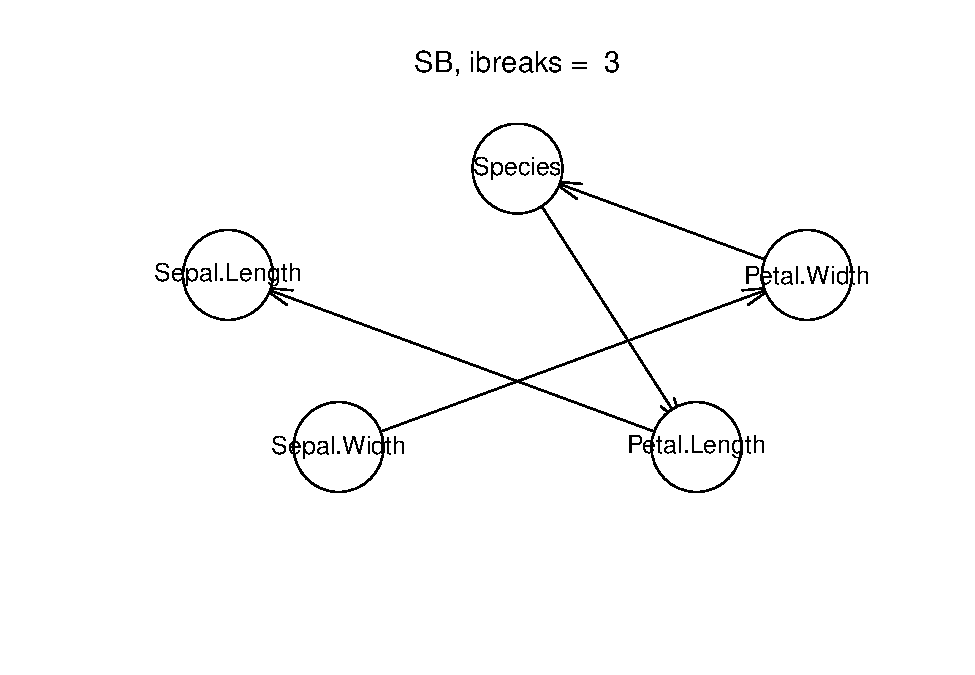
\includegraphics{BN_Ass2_files/figure-latex/unnamed-chunk-2-1.pdf}
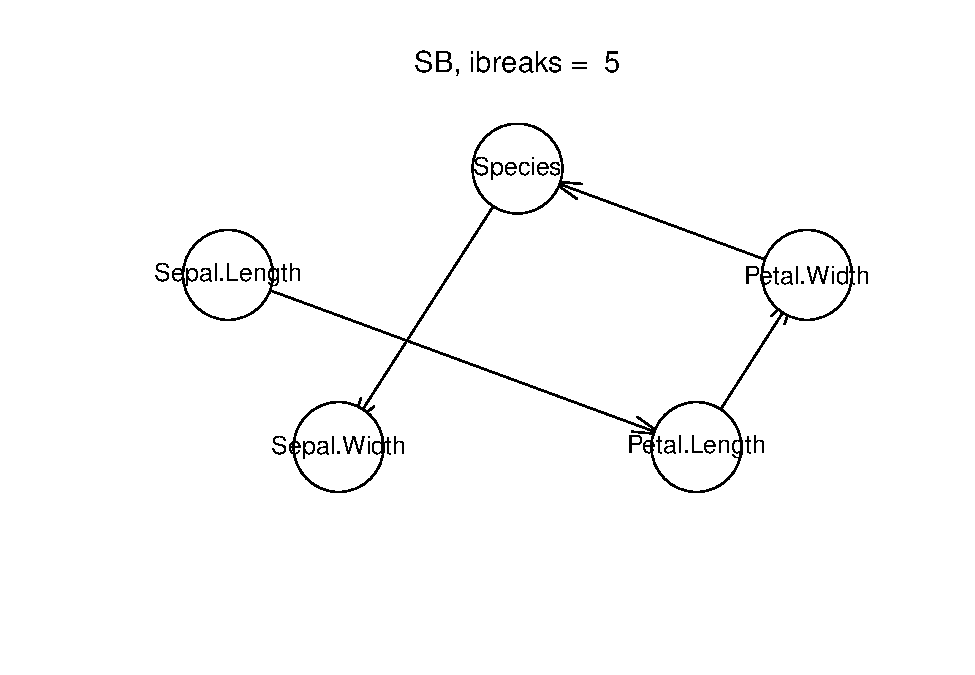
\includegraphics{BN_Ass2_files/figure-latex/unnamed-chunk-2-2.pdf}
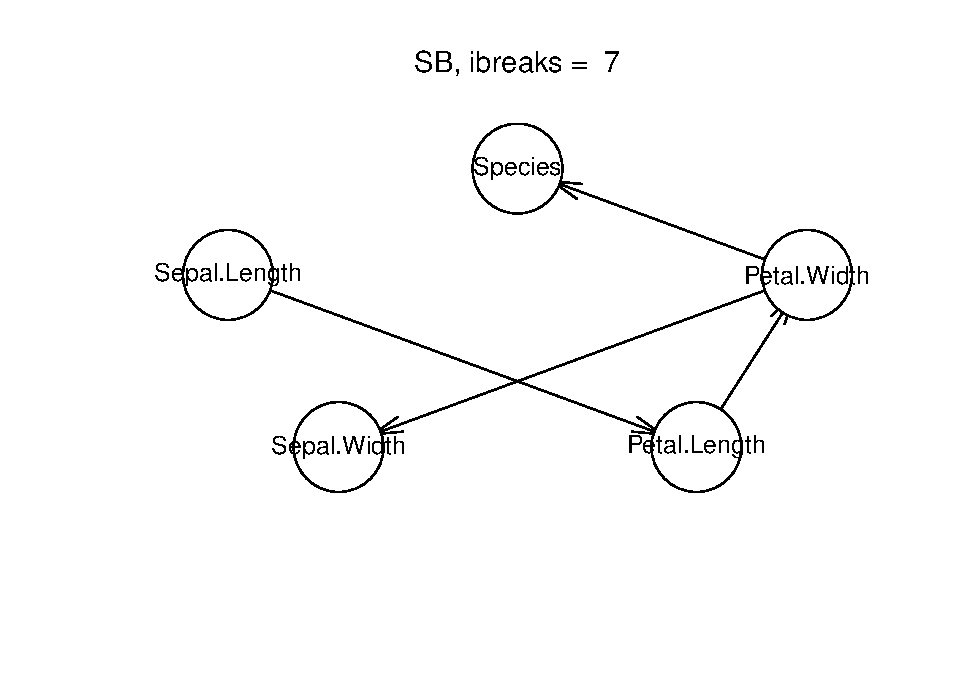
\includegraphics{BN_Ass2_files/figure-latex/unnamed-chunk-2-3.pdf}

\begin{Shaded}
\begin{Highlighting}[]
\NormalTok{for( bins in }\KeywordTok{c}\NormalTok{(}\DecValTok{3}\NormalTok{,}\DecValTok{5}\NormalTok{,}\DecValTok{7}\NormalTok{))\{}
\NormalTok{tmp=}\KeywordTok{discretize}\NormalTok{(iris[-}\DecValTok{5}\NormalTok{], }\DataTypeTok{method =} \StringTok{'hartemink'}\NormalTok{,}\DataTypeTok{ibreaks=}\NormalTok{bins) }
\NormalTok{NewIris =}\StringTok{ }\KeywordTok{cbind}\NormalTok{(tmp,iris[}\DecValTok{5}\NormalTok{]) }

\NormalTok{IrisNetcb <-}\StringTok{ }\KeywordTok{iamb}\NormalTok{(NewIris)}

\KeywordTok{plot}\NormalTok{(IrisNetcb, }\DataTypeTok{font.main =} \DecValTok{1}\NormalTok{, }\DataTypeTok{main =} \KeywordTok{paste}\NormalTok{(}\StringTok{"CB, ibreaks = "}\NormalTok{, bins))}

\NormalTok{\}}
\end{Highlighting}
\end{Shaded}

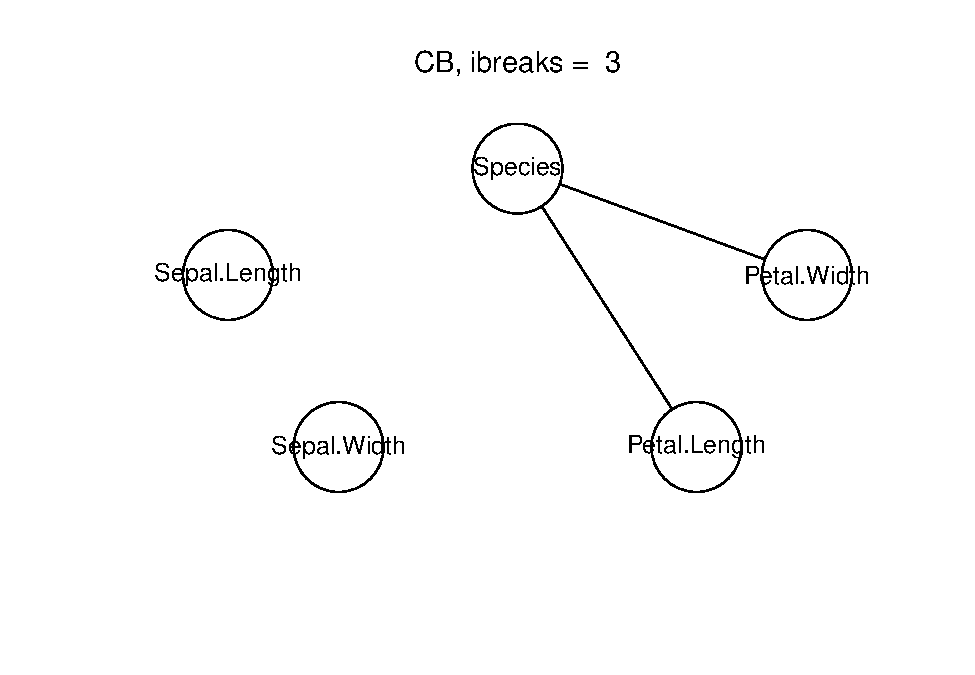
\includegraphics{BN_Ass2_files/figure-latex/unnamed-chunk-2-4.pdf}
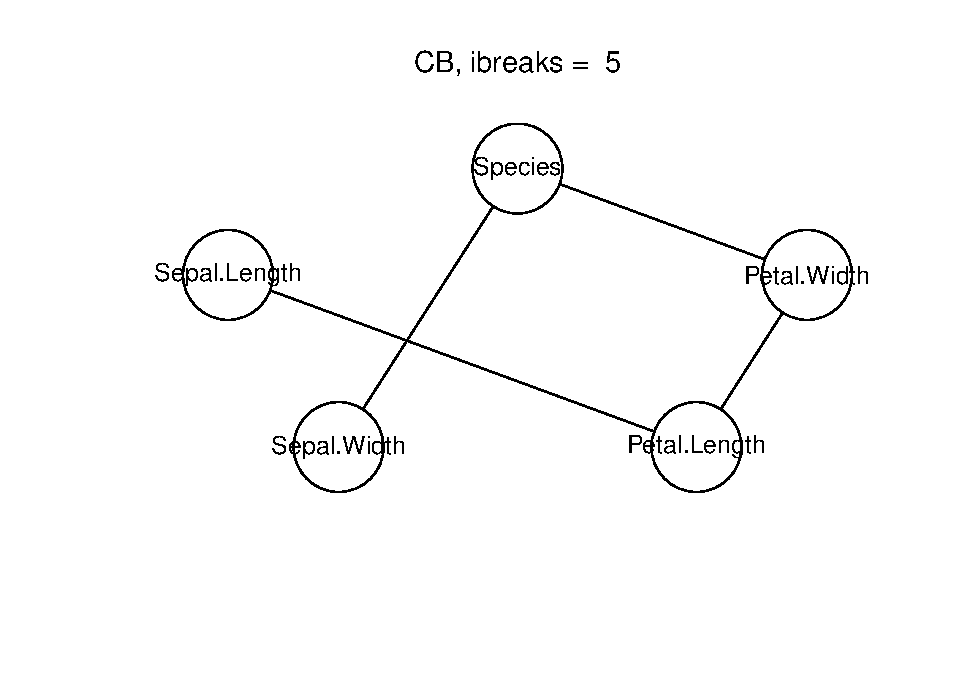
\includegraphics{BN_Ass2_files/figure-latex/unnamed-chunk-2-5.pdf}
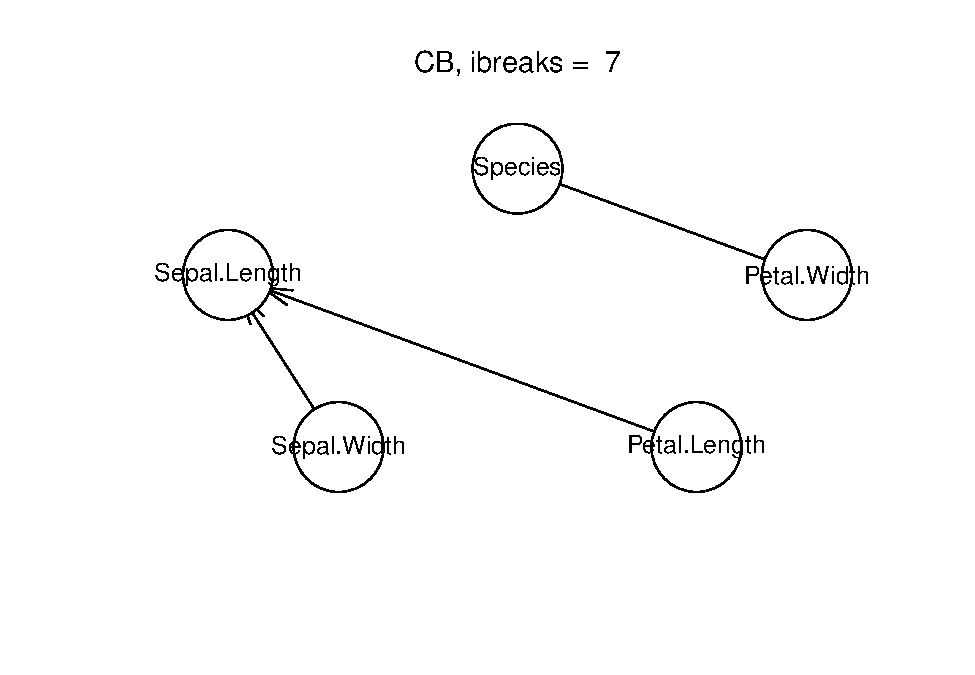
\includegraphics{BN_Ass2_files/figure-latex/unnamed-chunk-2-6.pdf}

\clearpage

constraint based:

\begin{itemize}
\item grow-shrink (GS())
\item incremental association markov blanket (IAMB())
\item Fast incremental association (FAST-IAMB())
\item interleaved incremental Association (inter-IAMB)
\end{itemize}

score based learning algos:

\begin{itemize}
\item Hill climbing (HC)
\item Tabu search (Tabu)
\end{itemize}

\newpage

\subsection{size of dataset}\label{size-of-dataset}

consider subsets of BC-dataset with different number of samples. both
classes of learning algios, compare results

\begin{Shaded}
\begin{Highlighting}[]
\NormalTok{a <-}\StringTok{ }\KeywordTok{read.csv}\NormalTok{(}\StringTok{'bc.csv'}\NormalTok{)}

\NormalTok{for(part in }\KeywordTok{c}\NormalTok{(}\DecValTok{10}\NormalTok{,}\DecValTok{2}\NormalTok{,}\DecValTok{1}\NormalTok{))\{}
    \NormalTok{ind =}\StringTok{ }\KeywordTok{sample}\NormalTok{(}\DecValTok{1}\NormalTok{:(}\KeywordTok{nrow}\NormalTok{(a)/part))}
    \NormalTok{BC <-}\StringTok{ }\NormalTok{a[ind,]}
    
    \NormalTok{BC_cbl <-}\StringTok{ }\KeywordTok{tabu}\NormalTok{(BC)}
    
    \KeywordTok{plot}\NormalTok{(BC_cbl , }\DataTypeTok{font.main =} \DecValTok{1}\NormalTok{, }\DataTypeTok{main =} \KeywordTok{paste}\NormalTok{(}\StringTok{"CB, every "}\NormalTok{, part, }\StringTok{"Datapoint"}\NormalTok{))}
\NormalTok{\}}
\end{Highlighting}
\end{Shaded}

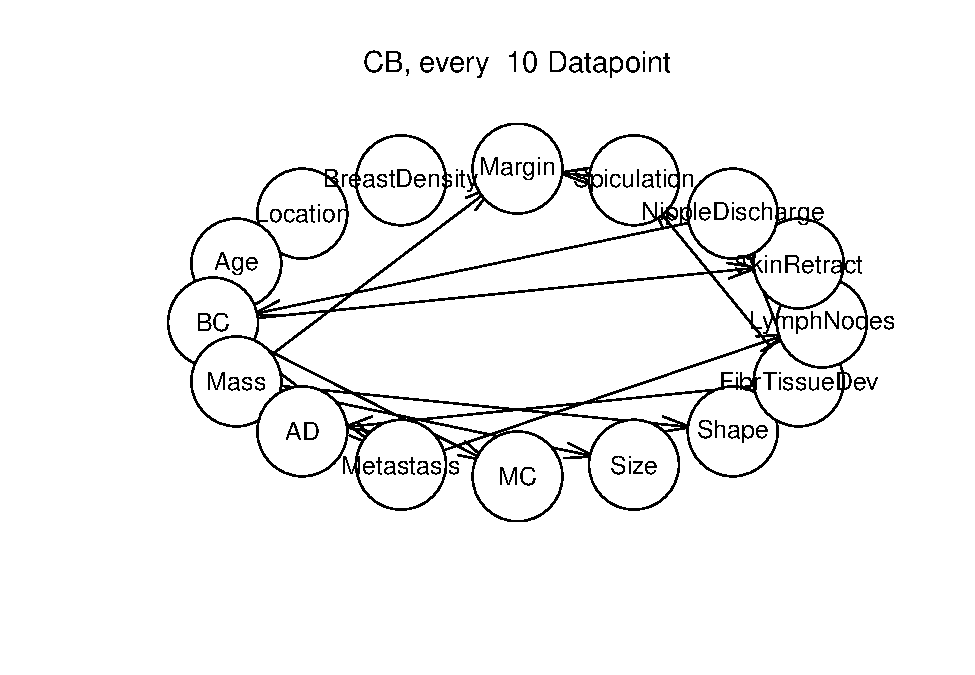
\includegraphics{BN_Ass2_files/figure-latex/unnamed-chunk-3-1.pdf}
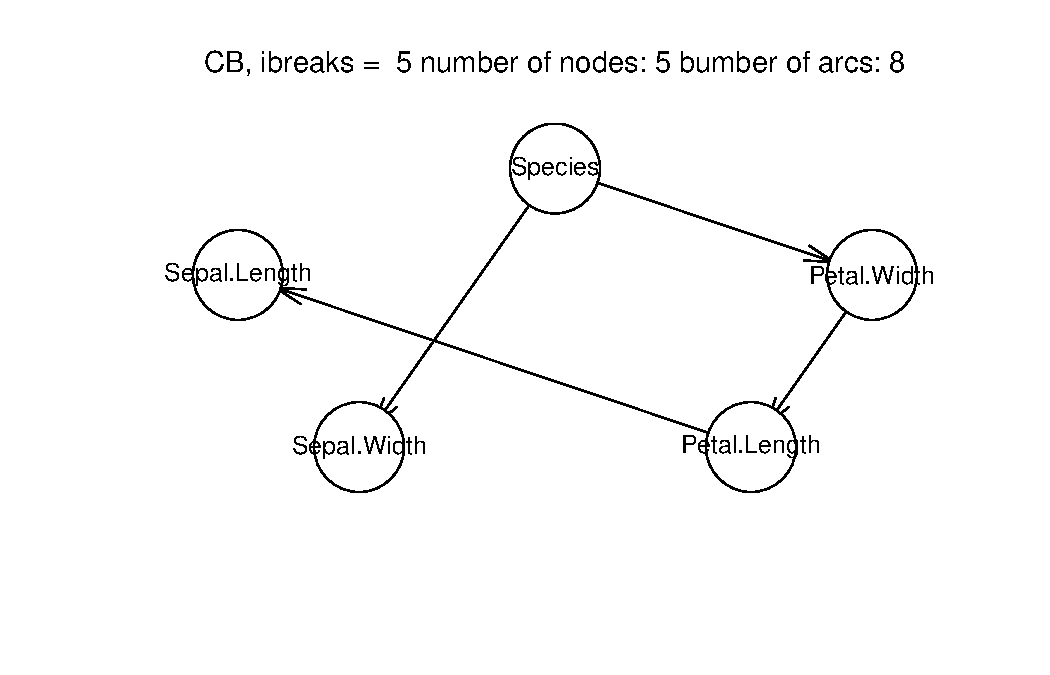
\includegraphics{BN_Ass2_files/figure-latex/unnamed-chunk-3-2.pdf}
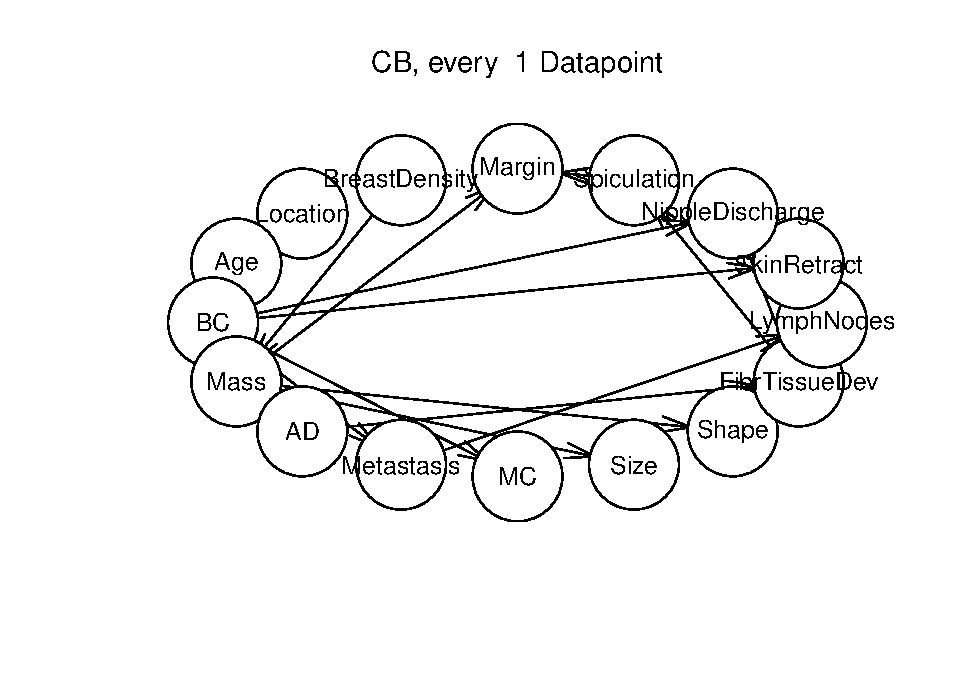
\includegraphics{BN_Ass2_files/figure-latex/unnamed-chunk-3-3.pdf}

\begin{Shaded}
\begin{Highlighting}[]
\NormalTok{for(part in }\KeywordTok{c}\NormalTok{(}\DecValTok{1}\NormalTok{,}\DecValTok{2}\NormalTok{,}\DecValTok{10}\NormalTok{))\{}
    \NormalTok{ind =}\StringTok{ }\KeywordTok{sample}\NormalTok{(}\DecValTok{1}\NormalTok{:(}\KeywordTok{nrow}\NormalTok{(a)/part))}
    \NormalTok{BC <-}\StringTok{ }\NormalTok{a[ind,]}
    
    \NormalTok{BC_sbl <-}\StringTok{ }\KeywordTok{iamb}\NormalTok{(BC)}

    \KeywordTok{plot}\NormalTok{(BC_sbl,  }\DataTypeTok{font.main =} \DecValTok{1}\NormalTok{, }\DataTypeTok{main =} \KeywordTok{paste}\NormalTok{(}\StringTok{"SB, every "}\NormalTok{, part, }\StringTok{"Datapoint"}\NormalTok{))}
\NormalTok{\}}
\end{Highlighting}
\end{Shaded}

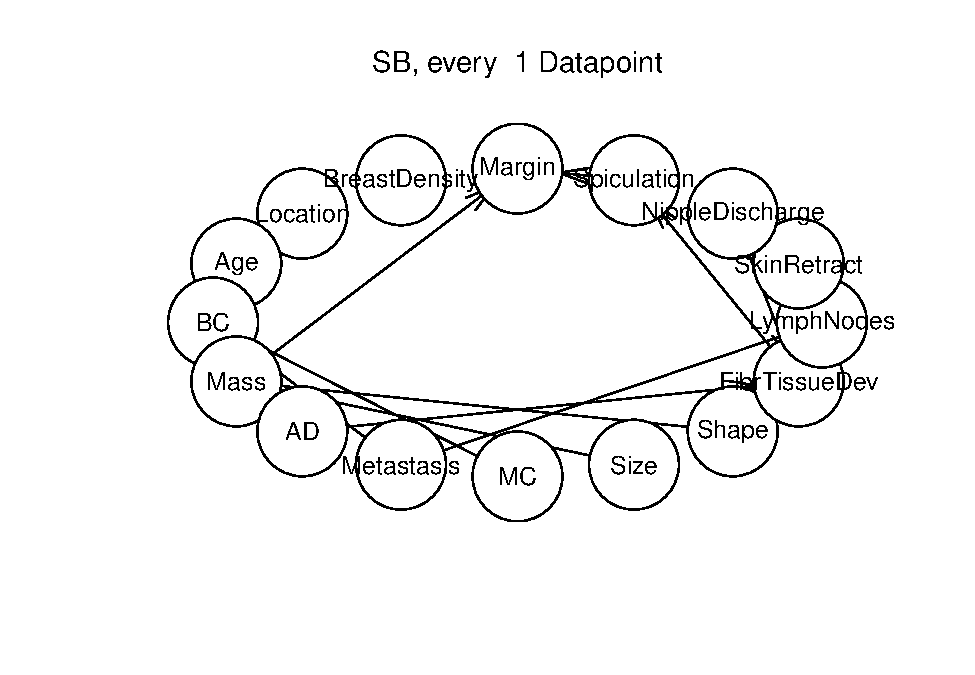
\includegraphics{BN_Ass2_files/figure-latex/unnamed-chunk-3-4.pdf}
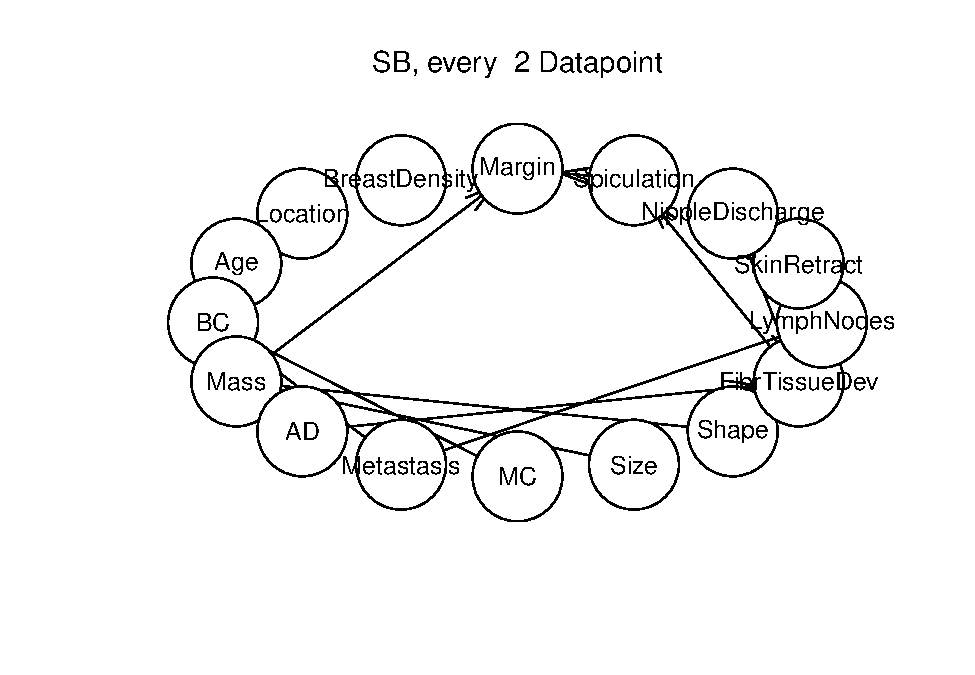
\includegraphics{BN_Ass2_files/figure-latex/unnamed-chunk-3-5.pdf}
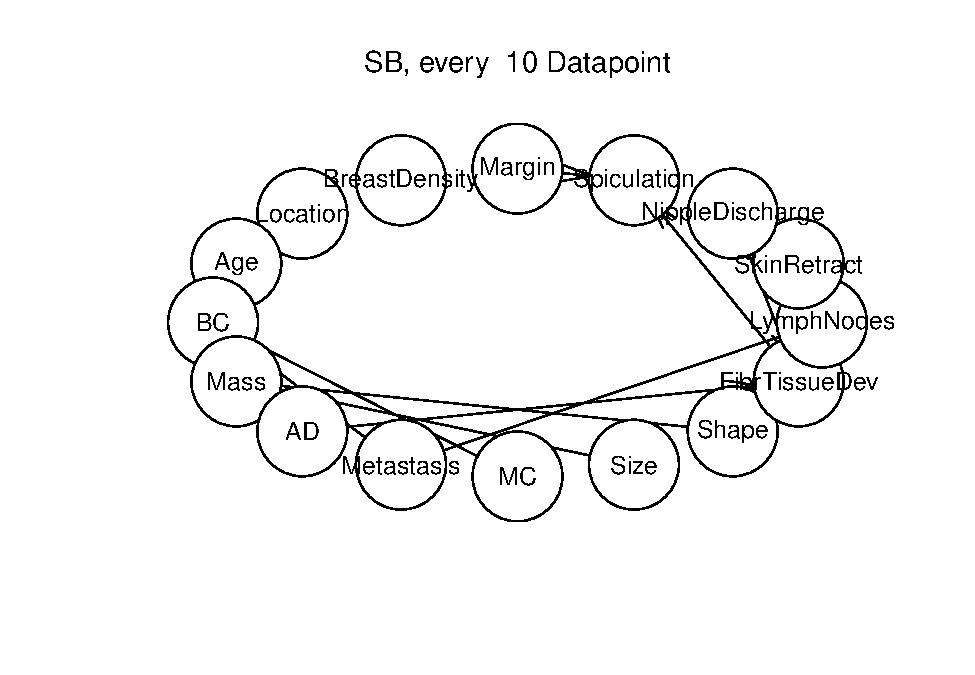
\includegraphics{BN_Ass2_files/figure-latex/unnamed-chunk-3-6.pdf}

\clearpage

\subsection{comparison to manually constructed bayes
network}\label{comparison-to-manually-constructed-bayes-network}

\begin{Shaded}
\begin{Highlighting}[]
\NormalTok{Tmp =}\StringTok{ }\KeywordTok{read.csv}\NormalTok{(}\StringTok{"nhl.csv"}\NormalTok{,}\DataTypeTok{nrows =} \DecValTok{5}\NormalTok{)}


\NormalTok{class =}\StringTok{ }\KeywordTok{rep}\NormalTok{(}\KeywordTok{list}\NormalTok{(}\StringTok{"factor"}\NormalTok{),}\KeywordTok{ncol}\NormalTok{(Tmp))}


\NormalTok{NHL =}\StringTok{ }\KeywordTok{read.csv}\NormalTok{(}\StringTok{"nhl.csv"}\NormalTok{,}\DataTypeTok{colClasses =} \NormalTok{class)}


\CommentTok{#impute(NHL[,c(2:ncol(Tmp))], fun=median)}
\CommentTok{#impute(NHL)}
\CommentTok{#impute(NHL[c(2:3),],fun=median)}

\NormalTok{Tmp2<-}\StringTok{ }\KeywordTok{complete.cases}\NormalTok{(NHL)}
\NormalTok{NHL <-}\StringTok{ }\NormalTok{NHL[Tmp2,]}


\NormalTok{NHLnet_sbl <-}\StringTok{ }\KeywordTok{tabu}\NormalTok{(NHL)}
\end{Highlighting}
\end{Shaded}

\begin{verbatim}
## Warning in check.data(x): variable AGE has levels that are not observed in
## the data.
\end{verbatim}

\begin{verbatim}
## Warning in check.data(x): variable BM_DEPRESSION has levels that are not
## observed in the data.
\end{verbatim}

\begin{Shaded}
\begin{Highlighting}[]
\NormalTok{NHLnet_cbl <-}\StringTok{ }\KeywordTok{iamb}\NormalTok{(NHL)}
\end{Highlighting}
\end{Shaded}

\begin{verbatim}
## Warning in check.data(x): variable AGE has levels that are not observed in
## the data.
\end{verbatim}

\begin{verbatim}
## Warning in check.data(x): variable BM_DEPRESSION has levels that are not
## observed in the data.
\end{verbatim}

\begin{Shaded}
\begin{Highlighting}[]
\KeywordTok{plot}\NormalTok{(NHLnet_sbl)}
\KeywordTok{title}\NormalTok{(}\StringTok{"NHL sbl"}\NormalTok{)}
\end{Highlighting}
\end{Shaded}

\begin{figure}[htbp]
\centering
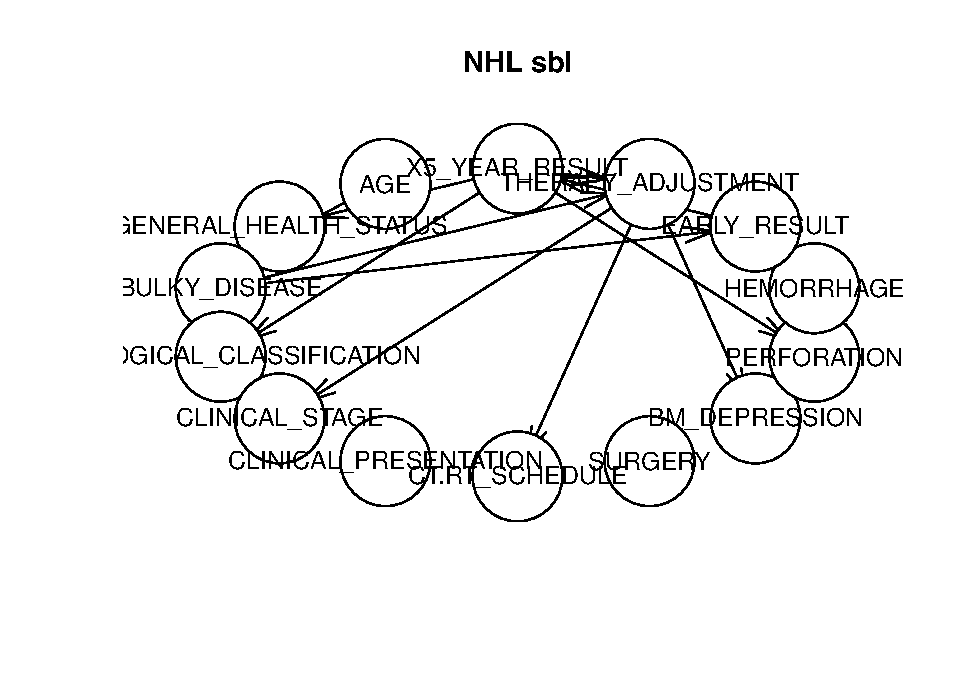
\includegraphics{BN_Ass2_files/figure-latex/unnamed-chunk-5-1.pdf}
\end{figure}

\begin{Shaded}
\begin{Highlighting}[]
\KeywordTok{plot}\NormalTok{(NHLnet_cbl)}
\KeywordTok{title}\NormalTok{(}\StringTok{"NHL cbl"}\NormalTok{)}
\end{Highlighting}
\end{Shaded}

\begin{figure}[htbp]
\centering
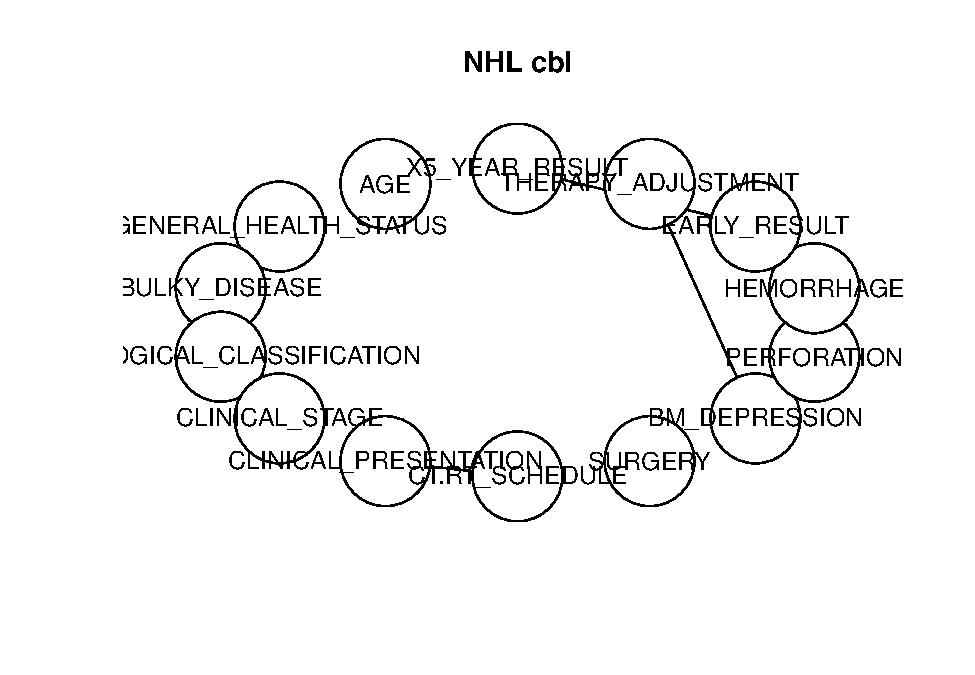
\includegraphics{BN_Ass2_files/figure-latex/unnamed-chunk-5-2.pdf}
\end{figure}

NHL dataset, liad column classes as factor (A.4)

missing data : probably median since mean desn't make sense for factors.

check for differences, unterschiedlcihe zahl nodes is ok.

\section{define measures for quality of a learning algorithm in terms of
a known bayes network structure, motivate
definition}\label{define-measures-for-quality-of-a-learning-algorithm-in-terms-of-a-known-bayes-network-structure-motivate-definition}

I have to be hones: I do not really understand that Question. Do the
authors suggest I find a measure that is original in describing the
quality of a bayesian Network? I'm sure that can't be true.

My measure for quality of the learning algorithm is Aruhga, which is the
Quotient between nodes and vertices.
\[Aruhga = \frac{Nodes}{Vertices}\]Arhuga is a binary measure with the
classes \{useful, not useful\}, depending on wether Aruhga falls inside
the interval {[}$\alpha , \beta${]}. $\alpha$ and $\beta$ are depending
heavily on the purpose and topic of the network and should normally be
defined by logical reasoning before constructing the network. However,
since the expert knowledge and necessary publications are not always
readily available, the author provides some default values with
$\alpha = 2.3$ and $\beta = 1.2/Nodes!$. Please note that Aruhga is a
measure of the connectivity of the network. values above alpha may
indicate that too many nodes are used, thus either weakening the
correlation between the single nodes OR bringing in Nodes that are not
relevant for each other. Networks with a value below beta indicate that
the network is highly connected which might reduce functionality and
also might point to a circular relationship between variables in the
real world that cannot be represented by a DAG.

\subsection{use measures to evaluate both classes of learning algs for
NHL
dataset}\label{use-measures-to-evaluate-both-classes-of-learning-algs-for-nhl-dataset}

\subsubsection{iris data set}\label{iris-data-set}

learnt with score learning algorithm: Aruhga = 5/4 = 1.25; beta = 1.2/5
= 0.002. learnt with Constraint based algorithm: Aruhga = 5/2 = 2.5;
beta = 1.2/5 = ,002

While the score learning algorithm scores well in terms of Aruhga, the
constraint based algorithm falls out of the default interval. Given that
sepal.length, sepal.width and petal.length are likely caused by the
species, we would say that the constraint based algorithm performs
poorly on this dataset.

\subsubsection{Breast cancer dataset}\label{breast-cancer-dataset}

nodes = 16, vertices = scoreFull =

\subsubsection{NHL}\label{nhl}

\subsection{compare margial prob distributions of learnt NHL bN with
those of the manually coinstructed
ones}\label{compare-margial-prob-distributions-of-learnt-nhl-bn-with-those-of-the-manually-coinstructed-ones}

since constraint based aslgorithms do not necessarily produce directed
graphs, we will only examine score based algorithms.

\begin{Shaded}
\begin{Highlighting}[]
\NormalTok{fittedNHL =}\StringTok{ }\KeywordTok{bn.fit}\NormalTok{(NHLnet_sbl,NHL)}
\end{Highlighting}
\end{Shaded}

\begin{verbatim}
## Warning in check.data(data): variable AGE has levels that are not observed
## in the data.
\end{verbatim}

\begin{verbatim}
## Warning in check.data(data): variable BM_DEPRESSION has levels that are
## not observed in the data.
\end{verbatim}

\begin{Shaded}
\begin{Highlighting}[]
\CommentTok{#fittedNHL2 = bn.fit(NHLnet_cbl,NHL)}
\CommentTok{# diagnostic BN structures}

\NormalTok{fittedNHL}
\end{Highlighting}
\end{Shaded}

\begin{verbatim}
## 
##   Bayesian network parameters
## 
##   Parameters of node AGE (multinomial distribution)
## 
## Conditional probability table:
##  
##           1          10          11           2           3           4 
## 0.009345794 0.224299065 0.084112150 0.000000000 0.046728972 0.028037383 
##           5           6           7           8           9 
## 0.130841121 0.121495327 0.140186916 0.084112150 0.130841121 
## 
##   Parameters of node GENERAL_HEALTH_STATUS (multinomial distribution)
## 
## Conditional probability table:
##  
##                      X5_YEAR_RESULT
## GENERAL_HEALTH_STATUS         1         2
##                     1 0.3965517 0.1632653
##                     2 0.6034483 0.5918367
##                     3 0.0000000 0.2448980
## 
##   Parameters of node BULKY_DISEASE (multinomial distribution)
## 
## Conditional probability table:
##  
##         1         2 
## 0.7383178 0.2616822 
## 
##   Parameters of node HISTOLOGICAL_CLASSIFICATION (multinomial distribution)
## 
## Conditional probability table:
##  
##                            X5_YEAR_RESULT
## HISTOLOGICAL_CLASSIFICATION          1          2
##                           1 0.63793103 0.18367347
##                           2 0.34482759 0.81632653
##                           3 0.01724138 0.00000000
## 
##   Parameters of node CLINICAL_STAGE (multinomial distribution)
## 
## Conditional probability table:
##  
##               THERAPY_ADJUSTMENT
## CLINICAL_STAGE          0          1
##              1 0.75555556 0.17647059
##              2 0.11111111 0.17647059
##              3 0.04444444 0.29411765
##              4 0.00000000 0.11764706
##              5 0.08888889 0.23529412
## 
##   Parameters of node CLINICAL_PRESENTATION (multinomial distribution)
## 
## Conditional probability table:
##  
##           1           2           3           4 
## 0.644859813 0.168224299 0.177570093 0.009345794 
## 
##   Parameters of node CT.RT_SCHEDULE (multinomial distribution)
## 
## Conditional probability table:
##  
##               THERAPY_ADJUSTMENT
## CT.RT_SCHEDULE          0          1
##              0 0.01111111 0.00000000
##              1 0.93333333 0.29411765
##              2 0.04444444 0.29411765
##              3 0.01111111 0.41176471
## 
##   Parameters of node SURGERY (multinomial distribution)
## 
## Conditional probability table:
##  
##          1          2          3 
## 0.79439252 0.14953271 0.05607477 
## 
##   Parameters of node BM_DEPRESSION (multinomial distribution)
## 
## Conditional probability table:
##  
##              THERAPY_ADJUSTMENT
## BM_DEPRESSION         0         1
##             1 1.0000000 0.0000000
##             2 0.0000000 0.8823529
##             3 0.0000000 0.1176471
##             9 0.0000000 0.0000000
## 
##   Parameters of node PERFORATION (multinomial distribution)
## 
## Conditional probability table:
##  
##            X5_YEAR_RESULT
## PERFORATION          1          2
##           1 1.00000000 0.93877551
##           2 0.00000000 0.06122449
## 
##   Parameters of node HEMORRHAGE (multinomial distribution)
## 
## Conditional probability table:
##  
##          1          2 
## 0.92523364 0.07476636 
## 
##   Parameters of node EARLY_RESULT (multinomial distribution)
## 
## Conditional probability table:
##  
##             BULKY_DISEASE
## EARLY_RESULT          1          2
##            1 0.89873418 0.50000000
##            2 0.03797468 0.25000000
##            3 0.03797468 0.03571429
##            4 0.02531646 0.21428571
## 
##   Parameters of node THERAPY_ADJUSTMENT (multinomial distribution)
## 
## Conditional probability table:
##  
## , , X5_YEAR_RESULT = 1
## 
##                   BULKY_DISEASE
## THERAPY_ADJUSTMENT         1         2
##                  0 1.0000000 0.5714286
##                  1 0.0000000 0.4285714
## 
## , , X5_YEAR_RESULT = 2
## 
##                   BULKY_DISEASE
## THERAPY_ADJUSTMENT         1         2
##                  0 0.8214286 0.5714286
##                  1 0.1785714 0.4285714
## 
## 
##   Parameters of node X5_YEAR_RESULT (multinomial distribution)
## 
## Conditional probability table:
##  
##               EARLY_RESULT
## X5_YEAR_RESULT         1         2         3         4
##              1 0.6705882 0.1000000 0.0000000 0.0000000
##              2 0.3294118 0.9000000 1.0000000 1.0000000
\end{verbatim}

\begin{Shaded}
\begin{Highlighting}[]
\CommentTok{#fittedNHL2}
\end{Highlighting}
\end{Shaded}

leanr bayes network from BN using sas or cb algo

\section{develop special purpose BN (NBN or TAN, see
.2)}\label{develop-special-purpose-bn-nbn-or-tan-see-.2}

\begin{Shaded}
\begin{Highlighting}[]
\NormalTok{netnb =}\StringTok{ }\KeywordTok{naive.bayes}\NormalTok{(a,}\StringTok{"BC"}\NormalTok{)}
\KeywordTok{plot}\NormalTok{(netnb)}
\end{Highlighting}
\end{Shaded}

\begin{figure}[htbp]
\centering
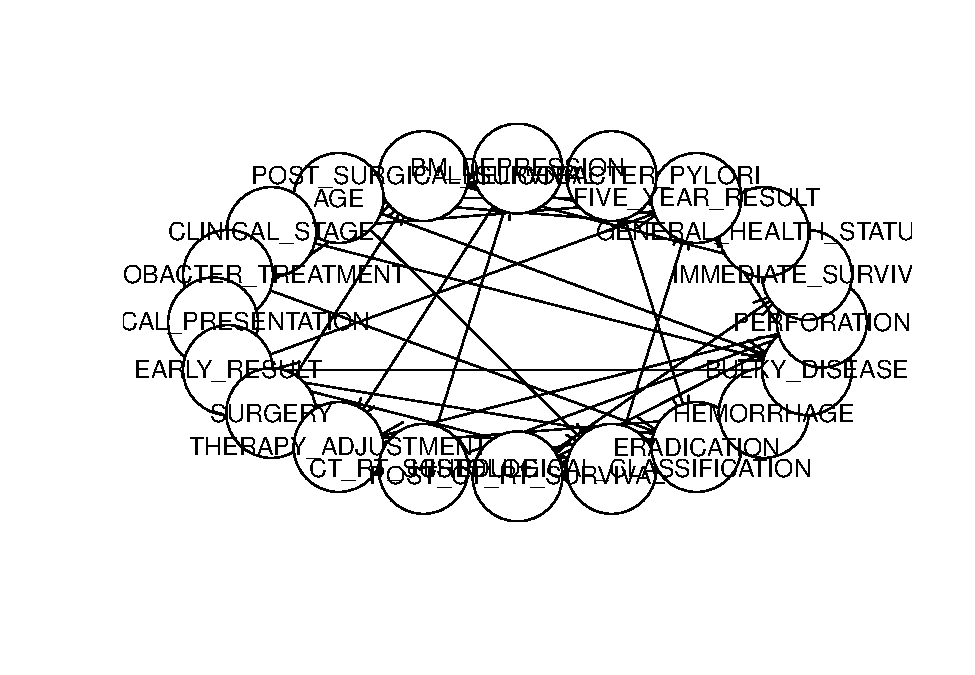
\includegraphics{BN_Ass2_files/figure-latex/unnamed-chunk-7-1.pdf}
\end{figure}

\begin{Shaded}
\begin{Highlighting}[]
\NormalTok{netnb2 <-}\StringTok{ }\KeywordTok{bn.fit}\NormalTok{(netnb,a)}
\CommentTok{#netnb2}
\CommentTok{#score(netnb,a)}
\CommentTok{#score(netnb2)}
\CommentTok{#score(a,BC_cbl)}
\end{Highlighting}
\end{Shaded}

\subsection{compare BN and SPBN with manually constructed network in
terms of network structure, goodnes of fit scores (lkikelohood,\ldots{})
and accuracy measures such as misclassification error and ROC
(B.2)}\label{compare-bn-and-spbn-with-manually-constructed-network-in-terms-of-network-structure-goodnes-of-fit-scores-lkikelohood-and-accuracy-measures-such-as-misclassification-error-and-roc-b.2}

\begin{Shaded}
\begin{Highlighting}[]
\NormalTok{netnb2 <-}\StringTok{ }\KeywordTok{bn.fit}\NormalTok{(netnb,a)}
\NormalTok{netnb2}
\end{Highlighting}
\end{Shaded}

\begin{verbatim}
## 
##   Bayesian network parameters
## 
##   Parameters of node BC (multinomial distribution)
## 
## Conditional probability table:
##  
##   Insitu Invasive       No 
##  0.14190  0.23615  0.62195 
## 
##   Parameters of node BreastDensity (multinomial distribution)
## 
## Conditional probability table:
##  
##              BC
## BreastDensity    Insitu  Invasive        No
##        high   0.3009161 0.3000212 0.3021143
##        low    0.1948555 0.1977557 0.2011416
##        medium 0.5042283 0.5022232 0.4967441
## 
##   Parameters of node Location (multinomial distribution)
## 
## Conditional probability table:
##  
##              BC
## Location         Insitu  Invasive        No
##   LolwOutQuad 0.2170543 0.2297269 0.2669829
##   LowInQuad   0.1976744 0.2576752 0.2602299
##   UpInQuad    0.2663848 0.2610629 0.2451966
##   UpOutQuad   0.3188865 0.2515350 0.2275906
## 
##   Parameters of node Age (multinomial distribution)
## 
## Conditional probability table:
##  
##        BC
## Age          Insitu    Invasive          No
##   <35   0.013389711 0.008680923 0.160784629
##   >75   0.136715997 0.131695956 0.156443444
##   35-49 0.311134602 0.168536947 0.263767184
##   50-74 0.538759690 0.691086174 0.419004743
## 
##   Parameters of node Mass (multinomial distribution)
## 
## Conditional probability table:
##  
##         BC
## Mass        Insitu  Invasive        No
##   Benign 0.4090909 0.1482109 0.1105394
##   Malign 0.3523608 0.6641965 0.0000000
##   No     0.2385483 0.1875926 0.8894606
## 
##   Parameters of node AD (multinomial distribution)
## 
## Conditional probability table:
##  
##      BC
## AD        Insitu   Invasive         No
##   No  0.70366455 0.54710989 0.94806656
##   Yes 0.29633545 0.45289011 0.05193344
## 
##   Parameters of node Metastasis (multinomial distribution)
## 
## Conditional probability table:
##  
##           BC
## Metastasis    Insitu  Invasive        No
##        no  0.8565891 0.1037476 1.0000000
##        yes 0.1434109 0.8962524 0.0000000
## 
##   Parameters of node MC (multinomial distribution)
## 
## Conditional probability table:
##  
##      BC
## MC        Insitu   Invasive         No
##   No  0.48731501 0.53080669 0.97202347
##   Yes 0.51268499 0.46919331 0.02797653
## 
##   Parameters of node Size (multinomial distribution)
## 
## Conditional probability table:
##  
##        BC
## Size        Insitu   Invasive         No
##   <1cm  0.37702607 0.39254711 0.90248412
##   >3cm  0.31606765 0.19839085 0.06961974
##   1-3cm 0.30690627 0.40906204 0.02789613
## 
##   Parameters of node Shape (multinomial distribution)
## 
## Conditional probability table:
##  
##            BC
## Shape            Insitu    Invasive          No
##   Irregular 0.278012685 0.501376244 0.006511777
##   Other     0.263918252 0.194791446 0.895329207
##   Oval      0.152924595 0.137836121 0.026047110
##   Round     0.305144468 0.165996189 0.072111906
## 
##   Parameters of node FibrTissueDev (multinomial distribution)
## 
## Conditional probability table:
##  
##              BC
## FibrTissueDev    Insitu  Invasive        No
##           No  0.5362932 0.4632649 0.6325267
##           Yes 0.4637068 0.5367351 0.3674733
## 
##   Parameters of node LymphNodes (multinomial distribution)
## 
## Conditional probability table:
##  
##           BC
## LymphNodes     Insitu   Invasive         No
##        no  0.80056378 0.23163244 0.90320765
##        yes 0.19943622 0.76836756 0.09679235
## 
##   Parameters of node SkinRetract (multinomial distribution)
## 
## Conditional probability table:
##  
##            BC
## SkinRetract    Insitu  Invasive        No
##         No  0.5574348 0.3823841 0.8419487
##         Yes 0.4425652 0.6176159 0.1580513
## 
##   Parameters of node NippleDischarge (multinomial distribution)
## 
## Conditional probability table:
##  
##                BC
## NippleDischarge    Insitu  Invasive        No
##             No  0.5821001 0.3900064 0.8455664
##             Yes 0.4178999 0.6099936 0.1544336
## 
##   Parameters of node Spiculation (multinomial distribution)
## 
## Conditional probability table:
##  
##            BC
## Spiculation    Insitu  Invasive        No
##         No  0.5775194 0.5386407 0.6277836
##         Yes 0.4224806 0.4613593 0.3722164
## 
##   Parameters of node Margin (multinomial distribution)
## 
## Conditional probability table:
##  
##               BC
## Margin            Insitu  Invasive        No
##   Ill-defined  0.5680056 0.7183993 0.3763968
##   Well-defined 0.4319944 0.2816007 0.6236032
\end{verbatim}

\begin{Shaded}
\begin{Highlighting}[]
\KeywordTok{score}\NormalTok{(netnb,a)}
\end{Highlighting}
\end{Shaded}

\begin{verbatim}
## [1] -214925.2
\end{verbatim}

\begin{Shaded}
\begin{Highlighting}[]
\NormalTok{nbncv <-}\StringTok{ }\KeywordTok{bn.cv}\NormalTok{(a,netnb,}\DataTypeTok{loss=}\StringTok{"logl"}\NormalTok{,}\DataTypeTok{loss.args =} \KeywordTok{list}\NormalTok{(}\DataTypeTok{target=}\StringTok{"BC"}\NormalTok{),}\DataTypeTok{debug=}\NormalTok{T)}
\end{Highlighting}
\end{Shaded}

\begin{verbatim}
## Warning in check.unused.args(extra.args, valid.args): unused argument(s):
## target
\end{verbatim}

\begin{verbatim}
## * splitting 20000 data in 10 subsets.
## ----------------------------------------------------------------
## * fitting the parameters of the network from the training sample.
## * applying the loss function to the data from the test sample.
##   > log-likelihood loss for node BC is 0.919676.
##   > log-likelihood loss for node BreastDensity is 1.039007.
##   > log-likelihood loss for node Location is 1.381308.
##   > log-likelihood loss for node Age is 1.167999.
##   > log-likelihood loss for node Mass is 0.578246.
##   > log-likelihood loss for node AD is 0.387564.
##   > log-likelihood loss for node Metastasis is 0.124055.
##   > log-likelihood loss for node MC is 0.362297.
##   > log-likelihood loss for node Size is 0.638856.
##   > log-likelihood loss for node Shape is 0.746732.
##   > log-likelihood loss for node FibrTissueDev is 0.660327.
##   > log-likelihood loss for node LymphNodes is 0.392187.
##   > log-likelihood loss for node SkinRetract is 0.519727.
##   > log-likelihood loss for node NippleDischarge is 0.521642.
##   > log-likelihood loss for node Spiculation is 0.667961.
##   > log-likelihood loss for node Margin is 0.654901.
##   @ total loss is 10.76249 .
## ----------------------------------------------------------------
## * fitting the parameters of the network from the training sample.
## * applying the loss function to the data from the test sample.
##   > log-likelihood loss for node BC is 0.893516.
##   > log-likelihood loss for node BreastDensity is 1.036432.
##   > log-likelihood loss for node Location is 1.382471.
##   > log-likelihood loss for node Age is 1.155939.
##   > log-likelihood loss for node Mass is 0.564805.
##   > log-likelihood loss for node AD is 0.364705.
##   > log-likelihood loss for node Metastasis is 0.145952.
##   > log-likelihood loss for node MC is 0.316122.
##   > log-likelihood loss for node Size is 0.631846.
##   > log-likelihood loss for node Shape is 0.729379.
##   > log-likelihood loss for node FibrTissueDev is 0.671738.
##   > log-likelihood loss for node LymphNodes is 0.407832.
##   > log-likelihood loss for node SkinRetract is 0.534846.
##   > log-likelihood loss for node NippleDischarge is 0.533331.
##   > log-likelihood loss for node Spiculation is 0.682359.
##   > log-likelihood loss for node Margin is 0.653261.
##   @ total loss is 10.70453 .
## ----------------------------------------------------------------
## * fitting the parameters of the network from the training sample.
## * applying the loss function to the data from the test sample.
##   > log-likelihood loss for node BC is 0.915643.
##   > log-likelihood loss for node BreastDensity is 1.022659.
##   > log-likelihood loss for node Location is 1.382281.
##   > log-likelihood loss for node Age is 1.142923.
##   > log-likelihood loss for node Mass is 0.568072.
##   > log-likelihood loss for node AD is 0.370244.
##   > log-likelihood loss for node Metastasis is 0.148668.
##   > log-likelihood loss for node MC is 0.355863.
##   > log-likelihood loss for node Size is 0.627118.
##   > log-likelihood loss for node Shape is 0.740264.
##   > log-likelihood loss for node FibrTissueDev is 0.657433.
##   > log-likelihood loss for node LymphNodes is 0.377287.
##   > log-likelihood loss for node SkinRetract is 0.505885.
##   > log-likelihood loss for node NippleDischarge is 0.495894.
##   > log-likelihood loss for node Spiculation is 0.657956.
##   > log-likelihood loss for node Margin is 0.646266.
##   @ total loss is 10.61446 .
## ----------------------------------------------------------------
## * fitting the parameters of the network from the training sample.
## * applying the loss function to the data from the test sample.
##   > log-likelihood loss for node BC is 0.915657.
##   > log-likelihood loss for node BreastDensity is 1.026515.
##   > log-likelihood loss for node Location is 1.383520.
##   > log-likelihood loss for node Age is 1.138271.
##   > log-likelihood loss for node Mass is 0.576120.
##   > log-likelihood loss for node AD is 0.372653.
##   > log-likelihood loss for node Metastasis is 0.127947.
##   > log-likelihood loss for node MC is 0.371117.
##   > log-likelihood loss for node Size is 0.649744.
##   > log-likelihood loss for node Shape is 0.767044.
##   > log-likelihood loss for node FibrTissueDev is 0.673687.
##   > log-likelihood loss for node LymphNodes is 0.374521.
##   > log-likelihood loss for node SkinRetract is 0.547325.
##   > log-likelihood loss for node NippleDischarge is 0.510130.
##   > log-likelihood loss for node Spiculation is 0.670490.
##   > log-likelihood loss for node Margin is 0.649255.
##   @ total loss is 10.75399 .
## ----------------------------------------------------------------
## * fitting the parameters of the network from the training sample.
## * applying the loss function to the data from the test sample.
##   > log-likelihood loss for node BC is 0.900075.
##   > log-likelihood loss for node BreastDensity is 1.016240.
##   > log-likelihood loss for node Location is 1.381208.
##   > log-likelihood loss for node Age is 1.159611.
##   > log-likelihood loss for node Mass is 0.537845.
##   > log-likelihood loss for node AD is 0.370768.
##   > log-likelihood loss for node Metastasis is 0.137597.
##   > log-likelihood loss for node MC is 0.321132.
##   > log-likelihood loss for node Size is 0.605181.
##   > log-likelihood loss for node Shape is 0.703885.
##   > log-likelihood loss for node FibrTissueDev is 0.663016.
##   > log-likelihood loss for node LymphNodes is 0.375928.
##   > log-likelihood loss for node SkinRetract is 0.502679.
##   > log-likelihood loss for node NippleDischarge is 0.517212.
##   > log-likelihood loss for node Spiculation is 0.662827.
##   > log-likelihood loss for node Margin is 0.641850.
##   @ total loss is 10.49705 .
## ----------------------------------------------------------------
## * fitting the parameters of the network from the training sample.
## * applying the loss function to the data from the test sample.
##   > log-likelihood loss for node BC is 0.925814.
##   > log-likelihood loss for node BreastDensity is 1.031562.
##   > log-likelihood loss for node Location is 1.387262.
##   > log-likelihood loss for node Age is 1.161452.
##   > log-likelihood loss for node Mass is 0.599065.
##   > log-likelihood loss for node AD is 0.381506.
##   > log-likelihood loss for node Metastasis is 0.142968.
##   > log-likelihood loss for node MC is 0.358106.
##   > log-likelihood loss for node Size is 0.662343.
##   > log-likelihood loss for node Shape is 0.772633.
##   > log-likelihood loss for node FibrTissueDev is 0.684539.
##   > log-likelihood loss for node LymphNodes is 0.401797.
##   > log-likelihood loss for node SkinRetract is 0.543047.
##   > log-likelihood loss for node NippleDischarge is 0.539979.
##   > log-likelihood loss for node Spiculation is 0.681120.
##   > log-likelihood loss for node Margin is 0.666037.
##   @ total loss is 10.93923 .
## ----------------------------------------------------------------
## * fitting the parameters of the network from the training sample.
## * applying the loss function to the data from the test sample.
##   > log-likelihood loss for node BC is 0.902563.
##   > log-likelihood loss for node BreastDensity is 1.033173.
##   > log-likelihood loss for node Location is 1.384384.
##   > log-likelihood loss for node Age is 1.145189.
##   > log-likelihood loss for node Mass is 0.571342.
##   > log-likelihood loss for node AD is 0.384618.
##   > log-likelihood loss for node Metastasis is 0.137036.
##   > log-likelihood loss for node MC is 0.317559.
##   > log-likelihood loss for node Size is 0.620296.
##   > log-likelihood loss for node Shape is 0.731096.
##   > log-likelihood loss for node FibrTissueDev is 0.673215.
##   > log-likelihood loss for node LymphNodes is 0.422698.
##   > log-likelihood loss for node SkinRetract is 0.517889.
##   > log-likelihood loss for node NippleDischarge is 0.525297.
##   > log-likelihood loss for node Spiculation is 0.670230.
##   > log-likelihood loss for node Margin is 0.651243.
##   @ total loss is 10.68783 .
## ----------------------------------------------------------------
## * fitting the parameters of the network from the training sample.
## * applying the loss function to the data from the test sample.
##   > log-likelihood loss for node BC is 0.906352.
##   > log-likelihood loss for node BreastDensity is 1.036702.
##   > log-likelihood loss for node Location is 1.384504.
##   > log-likelihood loss for node Age is 1.190130.
##   > log-likelihood loss for node Mass is 0.571520.
##   > log-likelihood loss for node AD is 0.359120.
##   > log-likelihood loss for node Metastasis is 0.143469.
##   > log-likelihood loss for node MC is 0.318990.
##   > log-likelihood loss for node Size is 0.654042.
##   > log-likelihood loss for node Shape is 0.746246.
##   > log-likelihood loss for node FibrTissueDev is 0.668176.
##   > log-likelihood loss for node LymphNodes is 0.394714.
##   > log-likelihood loss for node SkinRetract is 0.538348.
##   > log-likelihood loss for node NippleDischarge is 0.527464.
##   > log-likelihood loss for node Spiculation is 0.670680.
##   > log-likelihood loss for node Margin is 0.641574.
##   @ total loss is 10.75203 .
## ----------------------------------------------------------------
## * fitting the parameters of the network from the training sample.
## * applying the loss function to the data from the test sample.
##   > log-likelihood loss for node BC is 0.932720.
##   > log-likelihood loss for node BreastDensity is 1.039560.
##   > log-likelihood loss for node Location is 1.380445.
##   > log-likelihood loss for node Age is 1.163840.
##   > log-likelihood loss for node Mass is 0.594058.
##   > log-likelihood loss for node AD is 0.376309.
##   > log-likelihood loss for node Metastasis is 0.143458.
##   > log-likelihood loss for node MC is 0.338360.
##   > log-likelihood loss for node Size is 0.655879.
##   > log-likelihood loss for node Shape is 0.757259.
##   > log-likelihood loss for node FibrTissueDev is 0.674574.
##   > log-likelihood loss for node LymphNodes is 0.411048.
##   > log-likelihood loss for node SkinRetract is 0.520826.
##   > log-likelihood loss for node NippleDischarge is 0.529759.
##   > log-likelihood loss for node Spiculation is 0.668189.
##   > log-likelihood loss for node Margin is 0.648054.
##   @ total loss is 10.83434 .
## ----------------------------------------------------------------
## * fitting the parameters of the network from the training sample.
## * applying the loss function to the data from the test sample.
##   > log-likelihood loss for node BC is 0.922295.
##   > log-likelihood loss for node BreastDensity is 1.019785.
##   > log-likelihood loss for node Location is 1.382629.
##   > log-likelihood loss for node Age is 1.161628.
##   > log-likelihood loss for node Mass is 0.579984.
##   > log-likelihood loss for node AD is 0.392958.
##   > log-likelihood loss for node Metastasis is 0.120606.
##   > log-likelihood loss for node MC is 0.352155.
##   > log-likelihood loss for node Size is 0.648921.
##   > log-likelihood loss for node Shape is 0.744615.
##   > log-likelihood loss for node FibrTissueDev is 0.675616.
##   > log-likelihood loss for node LymphNodes is 0.408755.
##   > log-likelihood loss for node SkinRetract is 0.530315.
##   > log-likelihood loss for node NippleDischarge is 0.520983.
##   > log-likelihood loss for node Spiculation is 0.671986.
##   > log-likelihood loss for node Margin is 0.642909.
##   @ total loss is 10.77614 .
## ----------------------------------------------------------------
## * summary of the observed values for the loss function:
##    Min. 1st Qu.  Median    Mean 3rd Qu.    Max. 
##   10.50   10.69   10.75   10.73   10.77   10.94
\end{verbatim}

\begin{Shaded}
\begin{Highlighting}[]
\NormalTok{nbncv}
\end{Highlighting}
\end{Shaded}

\begin{verbatim}
## 
##   k-fold cross-validation for Bayesian networks
## 
##   target network structure:
##    [Naive Bayes Classifier]
##   number of subsets:                     10 
##   loss function:                         Log-Likelihood Loss (disc.) 
##   expected loss:                         10.73221
\end{verbatim}

\begin{Shaded}
\begin{Highlighting}[]
\NormalTok{bncv <-}\StringTok{ }\KeywordTok{bn.cv}\NormalTok{(a,BC_cbl,}\DataTypeTok{loss=}\StringTok{"logl"}\NormalTok{,}\DataTypeTok{loss.args =} \KeywordTok{list}\NormalTok{(}\DataTypeTok{target=}\StringTok{"BC"}\NormalTok{),}\DataTypeTok{debug=}\NormalTok{T)}
\end{Highlighting}
\end{Shaded}

\begin{verbatim}
## Warning in check.unused.args(extra.args, valid.args): unused argument(s):
## target
\end{verbatim}

\begin{verbatim}
## * splitting 20000 data in 10 subsets.
## ----------------------------------------------------------------
## * fitting the parameters of the network from the training sample.
## * applying the loss function to the data from the test sample.
##   > log-likelihood loss for node BreastDensity is 1.030255.
##   > log-likelihood loss for node Location is 1.384996.
##   > log-likelihood loss for node Age is 1.189759.
##   > log-likelihood loss for node BC is 0.879518.
##   > log-likelihood loss for node Mass is 0.574950.
##   > log-likelihood loss for node AD is 0.382096.
##   > log-likelihood loss for node Metastasis is 0.126285.
##   > log-likelihood loss for node MC is 0.335890.
##   > log-likelihood loss for node Size is 0.337169.
##   > log-likelihood loss for node Shape is 0.315042.
##   > log-likelihood loss for node FibrTissueDev is 0.623347.
##   > log-likelihood loss for node LymphNodes is 0.347303.
##   > log-likelihood loss for node SkinRetract is 0.418002.
##   > log-likelihood loss for node NippleDischarge is 0.446684.
##   > log-likelihood loss for node Spiculation is 0.486346.
##   > log-likelihood loss for node Margin is 0.170600.
##   @ total loss is 9.048242 .
## ----------------------------------------------------------------
## * fitting the parameters of the network from the training sample.
## * applying the loss function to the data from the test sample.
##   > log-likelihood loss for node BreastDensity is 1.033977.
##   > log-likelihood loss for node Location is 1.381462.
##   > log-likelihood loss for node Age is 1.201238.
##   > log-likelihood loss for node BC is 0.871718.
##   > log-likelihood loss for node Mass is 0.558205.
##   > log-likelihood loss for node AD is 0.364495.
##   > log-likelihood loss for node Metastasis is 0.127872.
##   > log-likelihood loss for node MC is 0.353685.
##   > log-likelihood loss for node Size is 0.332463.
##   > log-likelihood loss for node Shape is 0.301827.
##   > log-likelihood loss for node FibrTissueDev is 0.642236.
##   > log-likelihood loss for node LymphNodes is 0.332941.
##   > log-likelihood loss for node SkinRetract is 0.428725.
##   > log-likelihood loss for node NippleDischarge is 0.419254.
##   > log-likelihood loss for node Spiculation is 0.509892.
##   > log-likelihood loss for node Margin is 0.168618.
##   @ total loss is 9.028606 .
## ----------------------------------------------------------------
## * fitting the parameters of the network from the training sample.
## * applying the loss function to the data from the test sample.
##   > log-likelihood loss for node BreastDensity is 1.033977.
##   > log-likelihood loss for node Location is 1.379484.
##   > log-likelihood loss for node Age is 1.206621.
##   > log-likelihood loss for node BC is 0.866773.
##   > log-likelihood loss for node Mass is 0.571413.
##   > log-likelihood loss for node AD is 0.399776.
##   > log-likelihood loss for node Metastasis is 0.138560.
##   > log-likelihood loss for node MC is 0.343679.
##   > log-likelihood loss for node Size is 0.358865.
##   > log-likelihood loss for node Shape is 0.313509.
##   > log-likelihood loss for node FibrTissueDev is 0.625263.
##   > log-likelihood loss for node LymphNodes is 0.339830.
##   > log-likelihood loss for node SkinRetract is 0.426598.
##   > log-likelihood loss for node NippleDischarge is 0.445079.
##   > log-likelihood loss for node Spiculation is 0.474670.
##   > log-likelihood loss for node Margin is 0.197217.
##   @ total loss is 9.121313 .
## ----------------------------------------------------------------
## * fitting the parameters of the network from the training sample.
## * applying the loss function to the data from the test sample.
##   > log-likelihood loss for node BreastDensity is 1.016234.
##   > log-likelihood loss for node Location is 1.384000.
##   > log-likelihood loss for node Age is 1.207468.
##   > log-likelihood loss for node BC is 0.867267.
##   > log-likelihood loss for node Mass is 0.563447.
##   > log-likelihood loss for node AD is 0.356436.
##   > log-likelihood loss for node Metastasis is 0.145616.
##   > log-likelihood loss for node MC is 0.335520.
##   > log-likelihood loss for node Size is 0.342909.
##   > log-likelihood loss for node Shape is 0.328932.
##   > log-likelihood loss for node FibrTissueDev is 0.641469.
##   > log-likelihood loss for node LymphNodes is 0.347673.
##   > log-likelihood loss for node SkinRetract is 0.424056.
##   > log-likelihood loss for node NippleDischarge is 0.442624.
##   > log-likelihood loss for node Spiculation is 0.495071.
##   > log-likelihood loss for node Margin is 0.181371.
##   @ total loss is 9.080093 .
## ----------------------------------------------------------------
## * fitting the parameters of the network from the training sample.
## * applying the loss function to the data from the test sample.
##   > log-likelihood loss for node BreastDensity is 1.029002.
##   > log-likelihood loss for node Location is 1.382629.
##   > log-likelihood loss for node Age is 1.211219.
##   > log-likelihood loss for node BC is 0.876746.
##   > log-likelihood loss for node Mass is 0.568411.
##   > log-likelihood loss for node AD is 0.359373.
##   > log-likelihood loss for node Metastasis is 0.128843.
##   > log-likelihood loss for node MC is 0.334368.
##   > log-likelihood loss for node Size is 0.355771.
##   > log-likelihood loss for node Shape is 0.309850.
##   > log-likelihood loss for node FibrTissueDev is 0.624260.
##   > log-likelihood loss for node LymphNodes is 0.365184.
##   > log-likelihood loss for node SkinRetract is 0.435986.
##   > log-likelihood loss for node NippleDischarge is 0.425691.
##   > log-likelihood loss for node Spiculation is 0.474202.
##   > log-likelihood loss for node Margin is 0.165899.
##   @ total loss is 9.047435 .
## ----------------------------------------------------------------
## * fitting the parameters of the network from the training sample.
## * applying the loss function to the data from the test sample.
##   > log-likelihood loss for node BreastDensity is 1.028022.
##   > log-likelihood loss for node Location is 1.382318.
##   > log-likelihood loss for node Age is 1.231995.
##   > log-likelihood loss for node BC is 0.843704.
##   > log-likelihood loss for node Mass is 0.550439.
##   > log-likelihood loss for node AD is 0.385487.
##   > log-likelihood loss for node Metastasis is 0.148081.
##   > log-likelihood loss for node MC is 0.353395.
##   > log-likelihood loss for node Size is 0.334094.
##   > log-likelihood loss for node Shape is 0.287615.
##   > log-likelihood loss for node FibrTissueDev is 0.637738.
##   > log-likelihood loss for node LymphNodes is 0.352085.
##   > log-likelihood loss for node SkinRetract is 0.452968.
##   > log-likelihood loss for node NippleDischarge is 0.420431.
##   > log-likelihood loss for node Spiculation is 0.470118.
##   > log-likelihood loss for node Margin is 0.164146.
##   @ total loss is 9.042633 .
## ----------------------------------------------------------------
## * fitting the parameters of the network from the training sample.
## * applying the loss function to the data from the test sample.
##   > log-likelihood loss for node BreastDensity is 1.038228.
##   > log-likelihood loss for node Location is 1.385197.
##   > log-likelihood loss for node Age is 1.209743.
##   > log-likelihood loss for node BC is 0.850499.
##   > log-likelihood loss for node Mass is 0.570395.
##   > log-likelihood loss for node AD is 0.379295.
##   > log-likelihood loss for node Metastasis is 0.142859.
##   > log-likelihood loss for node MC is 0.351237.
##   > log-likelihood loss for node Size is 0.334331.
##   > log-likelihood loss for node Shape is 0.291664.
##   > log-likelihood loss for node FibrTissueDev is 0.635486.
##   > log-likelihood loss for node LymphNodes is 0.330478.
##   > log-likelihood loss for node SkinRetract is 0.445779.
##   > log-likelihood loss for node NippleDischarge is 0.427793.
##   > log-likelihood loss for node Spiculation is 0.471017.
##   > log-likelihood loss for node Margin is 0.175680.
##   @ total loss is 9.039681 .
## ----------------------------------------------------------------
## * fitting the parameters of the network from the training sample.
## * applying the loss function to the data from the test sample.
##   > log-likelihood loss for node BreastDensity is 1.021200.
##   > log-likelihood loss for node Location is 1.383945.
##   > log-likelihood loss for node Age is 1.210141.
##   > log-likelihood loss for node BC is 0.865670.
##   > log-likelihood loss for node Mass is 0.596426.
##   > log-likelihood loss for node AD is 0.381613.
##   > log-likelihood loss for node Metastasis is 0.145536.
##   > log-likelihood loss for node MC is 0.335588.
##   > log-likelihood loss for node Size is 0.349817.
##   > log-likelihood loss for node Shape is 0.305478.
##   > log-likelihood loss for node FibrTissueDev is 0.634805.
##   > log-likelihood loss for node LymphNodes is 0.347218.
##   > log-likelihood loss for node SkinRetract is 0.449045.
##   > log-likelihood loss for node NippleDischarge is 0.435177.
##   > log-likelihood loss for node Spiculation is 0.492143.
##   > log-likelihood loss for node Margin is 0.174433.
##   @ total loss is 9.128236 .
## ----------------------------------------------------------------
## * fitting the parameters of the network from the training sample.
## * applying the loss function to the data from the test sample.
##   > log-likelihood loss for node BreastDensity is 1.042566.
##   > log-likelihood loss for node Location is 1.383412.
##   > log-likelihood loss for node Age is 1.211938.
##   > log-likelihood loss for node BC is 0.840373.
##   > log-likelihood loss for node Mass is 0.561392.
##   > log-likelihood loss for node AD is 0.371731.
##   > log-likelihood loss for node Metastasis is 0.124461.
##   > log-likelihood loss for node MC is 0.323418.
##   > log-likelihood loss for node Size is 0.324547.
##   > log-likelihood loss for node Shape is 0.307674.
##   > log-likelihood loss for node FibrTissueDev is 0.641973.
##   > log-likelihood loss for node LymphNodes is 0.334497.
##   > log-likelihood loss for node SkinRetract is 0.441248.
##   > log-likelihood loss for node NippleDischarge is 0.432658.
##   > log-likelihood loss for node Spiculation is 0.477026.
##   > log-likelihood loss for node Margin is 0.178172.
##   @ total loss is 8.997087 .
## ----------------------------------------------------------------
## * fitting the parameters of the network from the training sample.
## * applying the loss function to the data from the test sample.
##   > log-likelihood loss for node BreastDensity is 1.026414.
##   > log-likelihood loss for node Location is 1.381599.
##   > log-likelihood loss for node Age is 1.223409.
##   > log-likelihood loss for node BC is 0.853779.
##   > log-likelihood loss for node Mass is 0.544816.
##   > log-likelihood loss for node AD is 0.380025.
##   > log-likelihood loss for node Metastasis is 0.143291.
##   > log-likelihood loss for node MC is 0.344351.
##   > log-likelihood loss for node Size is 0.344170.
##   > log-likelihood loss for node Shape is 0.296778.
##   > log-likelihood loss for node FibrTissueDev is 0.624222.
##   > log-likelihood loss for node LymphNodes is 0.350545.
##   > log-likelihood loss for node SkinRetract is 0.422709.
##   > log-likelihood loss for node NippleDischarge is 0.423236.
##   > log-likelihood loss for node Spiculation is 0.486101.
##   > log-likelihood loss for node Margin is 0.173377.
##   @ total loss is 9.018822 .
## ----------------------------------------------------------------
## * summary of the observed values for the loss function:
##    Min. 1st Qu.  Median    Mean 3rd Qu.    Max. 
##   8.997   9.031   9.045   9.055   9.072   9.128
\end{verbatim}

\begin{Shaded}
\begin{Highlighting}[]
\NormalTok{bncv}
\end{Highlighting}
\end{Shaded}

\begin{verbatim}
## 
##   k-fold cross-validation for Bayesian networks
## 
##   target network structure:
##    [BreastDensity][Age][BC|Age][Location|BC][Mass|BreastDensity:BC][AD|BC]
##    [Metastasis|BC][MC|BC][Size|Mass][Shape|Mass][FibrTissueDev|AD]
##    [LymphNodes|Metastasis][SkinRetract|BC:FibrTissueDev]
##    [NippleDischarge|BC:FibrTissueDev][Spiculation|FibrTissueDev]
##    [Margin|Mass:Spiculation]
##   number of subsets:                     10 
##   loss function:                         Log-Likelihood Loss (disc.) 
##   expected loss:                         9.055215
\end{verbatim}

\begin{Shaded}
\begin{Highlighting}[]
\NormalTok{nbncv <-}\StringTok{ }\KeywordTok{bn.cv}\NormalTok{(a,netnb,}\DataTypeTok{loss=}\StringTok{"pred"}\NormalTok{,}\DataTypeTok{loss.args =} \KeywordTok{list}\NormalTok{(}\DataTypeTok{target=}\StringTok{"BC"}\NormalTok{),}\DataTypeTok{debug=}\NormalTok{T)}
\end{Highlighting}
\end{Shaded}

\begin{verbatim}
## * splitting 20000 data in 10 subsets.
## ----------------------------------------------------------------
## * fitting the parameters of the network from the training sample.
## * applying the loss function to the data from the test sample.
##   > classification error for node BC is 0.139 .
##   @ total loss is 0.139 .
## ----------------------------------------------------------------
## * fitting the parameters of the network from the training sample.
## * applying the loss function to the data from the test sample.
##   > classification error for node BC is 0.134 .
##   @ total loss is 0.134 .
## ----------------------------------------------------------------
## * fitting the parameters of the network from the training sample.
## * applying the loss function to the data from the test sample.
##   > classification error for node BC is 0.1425 .
##   @ total loss is 0.1425 .
## ----------------------------------------------------------------
## * fitting the parameters of the network from the training sample.
## * applying the loss function to the data from the test sample.
##   > classification error for node BC is 0.1385 .
##   @ total loss is 0.1385 .
## ----------------------------------------------------------------
## * fitting the parameters of the network from the training sample.
## * applying the loss function to the data from the test sample.
##   > classification error for node BC is 0.146 .
##   @ total loss is 0.146 .
## ----------------------------------------------------------------
## * fitting the parameters of the network from the training sample.
## * applying the loss function to the data from the test sample.
##   > classification error for node BC is 0.1275 .
##   @ total loss is 0.1275 .
## ----------------------------------------------------------------
## * fitting the parameters of the network from the training sample.
## * applying the loss function to the data from the test sample.
##   > classification error for node BC is 0.146 .
##   @ total loss is 0.146 .
## ----------------------------------------------------------------
## * fitting the parameters of the network from the training sample.
## * applying the loss function to the data from the test sample.
##   > classification error for node BC is 0.144 .
##   @ total loss is 0.144 .
## ----------------------------------------------------------------
## * fitting the parameters of the network from the training sample.
## * applying the loss function to the data from the test sample.
##   > classification error for node BC is 0.1345 .
##   @ total loss is 0.1345 .
## ----------------------------------------------------------------
## * fitting the parameters of the network from the training sample.
## * applying the loss function to the data from the test sample.
##   > classification error for node BC is 0.1345 .
##   @ total loss is 0.1345 .
## ----------------------------------------------------------------
## * summary of the observed values for the loss function:
##    Min. 1st Qu.  Median    Mean 3rd Qu.    Max. 
##  0.1275  0.1345  0.1388  0.1386  0.1436  0.1460
\end{verbatim}

\begin{Shaded}
\begin{Highlighting}[]
\NormalTok{nbncv}
\end{Highlighting}
\end{Shaded}

\begin{verbatim}
## 
##   k-fold cross-validation for Bayesian networks
## 
##   target network structure:
##    [Naive Bayes Classifier]
##   number of subsets:                     10 
##   loss function:                         Classification Error 
##   training node:                         BC 
##   expected loss:                         0.13865
\end{verbatim}

\begin{Shaded}
\begin{Highlighting}[]
\NormalTok{bncv <-}\StringTok{ }\KeywordTok{bn.cv}\NormalTok{(a,BC_cbl,}\DataTypeTok{loss=}\StringTok{"pred"}\NormalTok{,}\DataTypeTok{loss.args =} \KeywordTok{list}\NormalTok{(}\DataTypeTok{target=}\StringTok{"BC"}\NormalTok{),}\DataTypeTok{debug=}\NormalTok{T)}
\end{Highlighting}
\end{Shaded}

\begin{verbatim}
## * splitting 20000 data in 10 subsets.
## ----------------------------------------------------------------
## * fitting the parameters of the network from the training sample.
## * applying the loss function to the data from the test sample.
##   > classification error for node BC is 0.3965 .
##   @ total loss is 0.3965 .
## ----------------------------------------------------------------
## * fitting the parameters of the network from the training sample.
## * applying the loss function to the data from the test sample.
##   > classification error for node BC is 0.3815 .
##   @ total loss is 0.3815 .
## ----------------------------------------------------------------
## * fitting the parameters of the network from the training sample.
## * applying the loss function to the data from the test sample.
##   > classification error for node BC is 0.376 .
##   @ total loss is 0.376 .
## ----------------------------------------------------------------
## * fitting the parameters of the network from the training sample.
## * applying the loss function to the data from the test sample.
##   > classification error for node BC is 0.374 .
##   @ total loss is 0.374 .
## ----------------------------------------------------------------
## * fitting the parameters of the network from the training sample.
## * applying the loss function to the data from the test sample.
##   > classification error for node BC is 0.3815 .
##   @ total loss is 0.3815 .
## ----------------------------------------------------------------
## * fitting the parameters of the network from the training sample.
## * applying the loss function to the data from the test sample.
##   > classification error for node BC is 0.375 .
##   @ total loss is 0.375 .
## ----------------------------------------------------------------
## * fitting the parameters of the network from the training sample.
## * applying the loss function to the data from the test sample.
##   > classification error for node BC is 0.3785 .
##   @ total loss is 0.3785 .
## ----------------------------------------------------------------
## * fitting the parameters of the network from the training sample.
## * applying the loss function to the data from the test sample.
##   > classification error for node BC is 0.362 .
##   @ total loss is 0.362 .
## ----------------------------------------------------------------
## * fitting the parameters of the network from the training sample.
## * applying the loss function to the data from the test sample.
##   > classification error for node BC is 0.38 .
##   @ total loss is 0.38 .
## ----------------------------------------------------------------
## * fitting the parameters of the network from the training sample.
## * applying the loss function to the data from the test sample.
##   > classification error for node BC is 0.3755 .
##   @ total loss is 0.3755 .
## ----------------------------------------------------------------
## * summary of the observed values for the loss function:
##    Min. 1st Qu.  Median    Mean 3rd Qu.    Max. 
##  0.3620  0.3751  0.3772  0.3780  0.3811  0.3965
\end{verbatim}

\begin{Shaded}
\begin{Highlighting}[]
\NormalTok{bncv}
\end{Highlighting}
\end{Shaded}

\begin{verbatim}
## 
##   k-fold cross-validation for Bayesian networks
## 
##   target network structure:
##    [BreastDensity][Age][BC|Age][Location|BC][Mass|BreastDensity:BC][AD|BC]
##    [Metastasis|BC][MC|BC][Size|Mass][Shape|Mass][FibrTissueDev|AD]
##    [LymphNodes|Metastasis][SkinRetract|BC:FibrTissueDev]
##    [NippleDischarge|BC:FibrTissueDev][Spiculation|FibrTissueDev]
##    [Margin|Mass:Spiculation]
##   number of subsets:                     10 
##   loss function:                         Classification Error 
##   training node:                         BC 
##   expected loss:                         0.37805
\end{verbatim}

Read in manually constructed network:

\begin{Shaded}
\begin{Highlighting}[]
\NormalTok{manual =}\StringTok{ }\KeywordTok{read.net}\NormalTok{(}\StringTok{"bc.net"}\NormalTok{)}

\CommentTok{#manual}

\CommentTok{#manNet = bn.fit(manual,a)}
\KeywordTok{names}\NormalTok{(manual)}
\end{Highlighting}
\end{Shaded}

\begin{verbatim}
##  [1] "MC"              "Spiculation"     "Location"       
##  [4] "Age"             "LymphNodes"      "SkinRetract"    
##  [7] "Shape"           "Size"            "BC"             
## [10] "FibrTissueDev"   "BreastDensity"   "Margin"         
## [13] "NippleDischarge" "AD"              "Metastasis"     
## [16] "Mass"
\end{verbatim}

\begin{Shaded}
\begin{Highlighting}[]
\KeywordTok{names}\NormalTok{(BC_cbl)}
\end{Highlighting}
\end{Shaded}

\begin{verbatim}
## [1] "learning" "nodes"    "arcs"
\end{verbatim}

\begin{Shaded}
\begin{Highlighting}[]
\KeywordTok{typeof}\NormalTok{(manual)}
\end{Highlighting}
\end{Shaded}

\begin{verbatim}
## [1] "list"
\end{verbatim}

\begin{Shaded}
\begin{Highlighting}[]
\KeywordTok{typeof}\NormalTok{(BC_cbl)}
\end{Highlighting}
\end{Shaded}

\begin{verbatim}
## [1] "list"
\end{verbatim}

\begin{Shaded}
\begin{Highlighting}[]
\NormalTok{test <-}\StringTok{ }\KeywordTok{bn.net}\NormalTok{(manual)}
\KeywordTok{plot}\NormalTok{(test)}
\end{Highlighting}
\end{Shaded}

\begin{figure}[htbp]
\centering
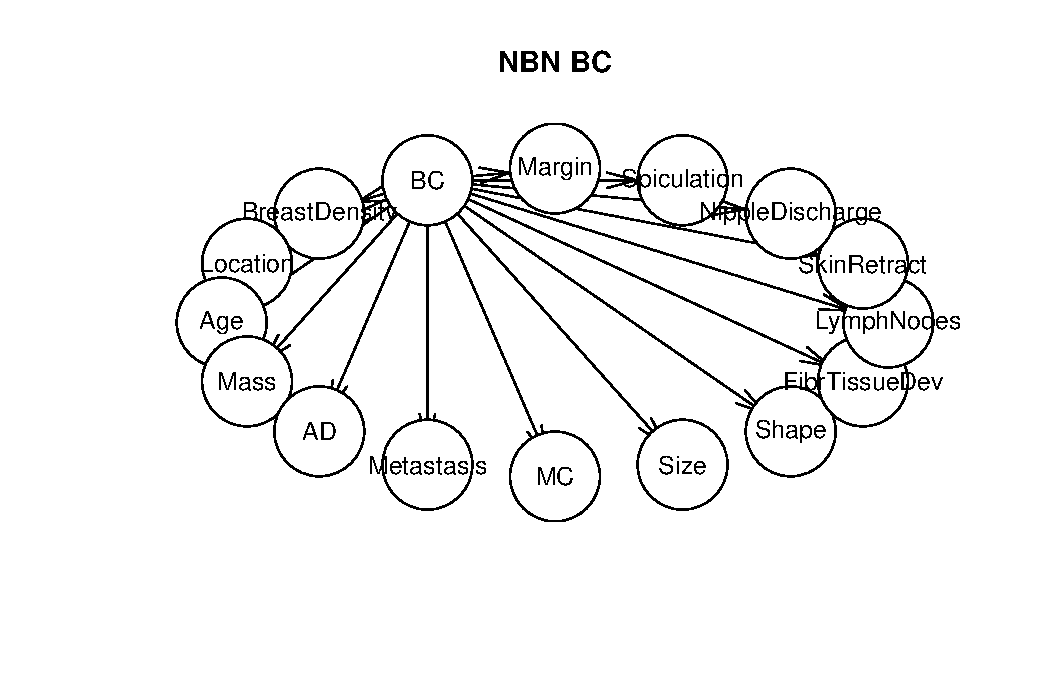
\includegraphics{BN_Ass2_files/figure-latex/unnamed-chunk-9-1.pdf}
\end{figure}

\begin{Shaded}
\begin{Highlighting}[]
\NormalTok{bncv <-}\StringTok{ }\KeywordTok{bn.cv}\NormalTok{(a,test,}\DataTypeTok{loss=}\StringTok{"pred"}\NormalTok{,}\DataTypeTok{loss.args =} \KeywordTok{list}\NormalTok{(}\DataTypeTok{target=}\StringTok{"BC"}\NormalTok{),}\DataTypeTok{debug=}\NormalTok{T)}
\end{Highlighting}
\end{Shaded}

\begin{verbatim}
## * splitting 20000 data in 10 subsets.
## ----------------------------------------------------------------
## * fitting the parameters of the network from the training sample.
## * applying the loss function to the data from the test sample.
##   > classification error for node BC is 0.3675 .
##   @ total loss is 0.3675 .
## ----------------------------------------------------------------
## * fitting the parameters of the network from the training sample.
## * applying the loss function to the data from the test sample.
##   > classification error for node BC is 0.3785 .
##   @ total loss is 0.3785 .
## ----------------------------------------------------------------
## * fitting the parameters of the network from the training sample.
## * applying the loss function to the data from the test sample.
##   > classification error for node BC is 0.3765 .
##   @ total loss is 0.3765 .
## ----------------------------------------------------------------
## * fitting the parameters of the network from the training sample.
## * applying the loss function to the data from the test sample.
##   > classification error for node BC is 0.3655 .
##   @ total loss is 0.3655 .
## ----------------------------------------------------------------
## * fitting the parameters of the network from the training sample.
## * applying the loss function to the data from the test sample.
##   > classification error for node BC is 0.366 .
##   @ total loss is 0.366 .
## ----------------------------------------------------------------
## * fitting the parameters of the network from the training sample.
## * applying the loss function to the data from the test sample.
##   > classification error for node BC is 0.3825 .
##   @ total loss is 0.3825 .
## ----------------------------------------------------------------
## * fitting the parameters of the network from the training sample.
## * applying the loss function to the data from the test sample.
##   > classification error for node BC is 0.3835 .
##   @ total loss is 0.3835 .
## ----------------------------------------------------------------
## * fitting the parameters of the network from the training sample.
## * applying the loss function to the data from the test sample.
##   > classification error for node BC is 0.3855 .
##   @ total loss is 0.3855 .
## ----------------------------------------------------------------
## * fitting the parameters of the network from the training sample.
## * applying the loss function to the data from the test sample.
##   > classification error for node BC is 0.3835 .
##   @ total loss is 0.3835 .
## ----------------------------------------------------------------
## * fitting the parameters of the network from the training sample.
## * applying the loss function to the data from the test sample.
##   > classification error for node BC is 0.3915 .
##   @ total loss is 0.3915 .
## ----------------------------------------------------------------
## * summary of the observed values for the loss function:
##    Min. 1st Qu.  Median    Mean 3rd Qu.    Max. 
##  0.3655  0.3698  0.3805  0.3780  0.3835  0.3915
\end{verbatim}

\begin{Shaded}
\begin{Highlighting}[]
\CommentTok{#manbncv <- bn.cv(a,manual,loss="logl",loss.args = list(target="BC"),debug=T)}
\CommentTok{#manbncv}
\end{Highlighting}
\end{Shaded}

library(ROCR),
\footnote{Tobias Sing, Oliver Sander, Niko Beerenwinkel, Thomas Lengauer.
ROCR: visualizing classifier performance in R.
Bioinformatics 21(20):3940-3941 (2005).} \cite{Sing2005} Sing et al.
(2005)

\section{Attachment A}\label{attachment-a}

\subsection{Iris dataset}\label{iris-dataset}

\subsubsection{other discretizations:}\label{other-discretizations}

\begin{Shaded}
\begin{Highlighting}[]
\NormalTok{NewIris <-}\StringTok{  }\KeywordTok{discretize}\NormalTok{(iris, }\DataTypeTok{method =} \StringTok{'interval'}\NormalTok{, }\DataTypeTok{breaks =} \DecValTok{3}\NormalTok{, }\DataTypeTok{ibreaks =} \DecValTok{3}\NormalTok{)}
\end{Highlighting}
\end{Shaded}

\begin{verbatim}
## Warning in check.unused.args(extra.args,
## discretization.extra.args[[method]]): unused argument(s): ibreaks
\end{verbatim}

\begin{Shaded}
\begin{Highlighting}[]
\NormalTok{NewIris1 <-}\StringTok{  }\KeywordTok{discretize}\NormalTok{(iris, }\DataTypeTok{method =} \StringTok{'interval'}\NormalTok{, }\DataTypeTok{breaks =} \DecValTok{100}\NormalTok{, }\DataTypeTok{ibreaks =} \DecValTok{10}\NormalTok{)}
\end{Highlighting}
\end{Shaded}

\begin{verbatim}
## Warning in check.unused.args(extra.args,
## discretization.extra.args[[method]]): unused argument(s): ibreaks
\end{verbatim}

\begin{Shaded}
\begin{Highlighting}[]
\NormalTok{NewIrisNetHc <-}\StringTok{ }\KeywordTok{tabu}\NormalTok{(NewIris)}
\NormalTok{NewIrisNetGs <-}\StringTok{ }\KeywordTok{iamb}\NormalTok{(NewIris)}

\NormalTok{NewIrisNetHc}
\end{Highlighting}
\end{Shaded}

\begin{verbatim}
## 
##   Bayesian network learned via Score-based methods
## 
##   model:
##    [Sepal.Width][Petal.Width|Sepal.Width][Species|Petal.Width]
##    [Petal.Length|Species][Sepal.Length|Petal.Length]
##   nodes:                                 5 
##   arcs:                                  4 
##     undirected arcs:                     0 
##     directed arcs:                       4 
##   average markov blanket size:           1.60 
##   average neighbourhood size:            1.60 
##   average branching factor:              0.80 
## 
##   learning algorithm:                    Tabu Search 
##   score:                                 BIC (disc.) 
##   penalization coefficient:              2.505318 
##   tests used in the learning procedure:  114 
##   optimized:                             TRUE
\end{verbatim}

\begin{Shaded}
\begin{Highlighting}[]
\NormalTok{NewIrisNetGs}
\end{Highlighting}
\end{Shaded}

\begin{verbatim}
## 
##   Bayesian network learned via Constraint-based methods
## 
##   model:
##     [undirected graph]
##   nodes:                                 5 
##   arcs:                                  2 
##     undirected arcs:                     2 
##     directed arcs:                       0 
##   average markov blanket size:           0.80 
##   average neighbourhood size:            0.80 
##   average branching factor:              0.00 
## 
##   learning algorithm:                    IAMB 
##   conditional independence test:         Mutual Information (disc.) 
##   alpha threshold:                       0.05 
##   tests used in the learning procedure:  32 
##   optimized:                             TRUE
\end{verbatim}

\begin{Shaded}
\begin{Highlighting}[]
\KeywordTok{plot}\NormalTok{(NewIrisNetHc)}
\end{Highlighting}
\end{Shaded}

\begin{figure}[htbp]
\centering
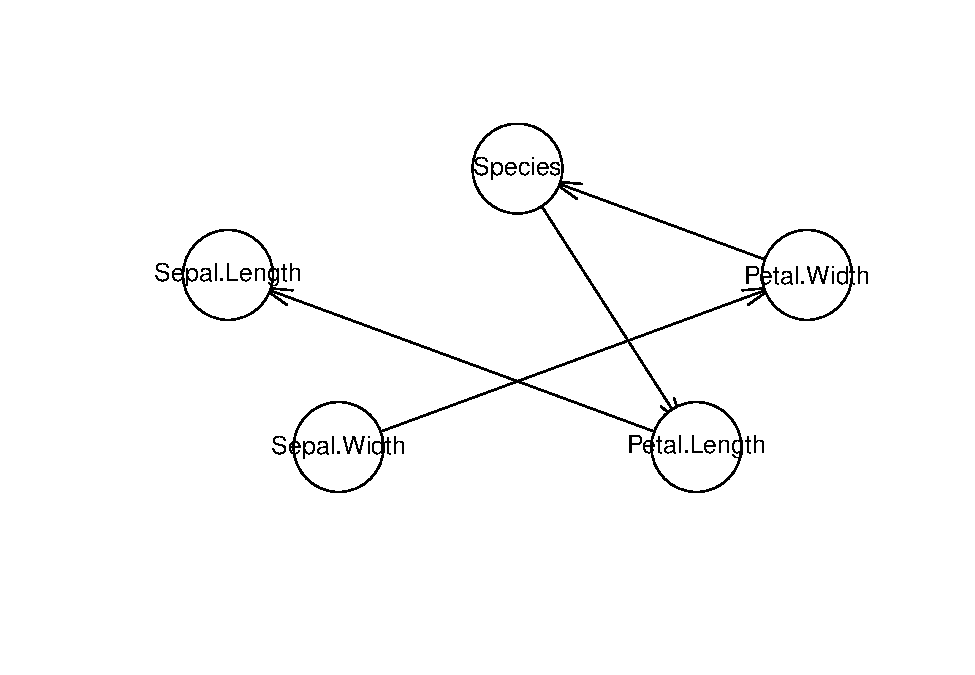
\includegraphics{BN_Ass2_files/figure-latex/unnamed-chunk-12-1.pdf}
\end{figure}

\begin{Shaded}
\begin{Highlighting}[]
\KeywordTok{plot}\NormalTok{(NewIrisNetGs)}
\end{Highlighting}
\end{Shaded}

\begin{figure}[htbp]
\centering
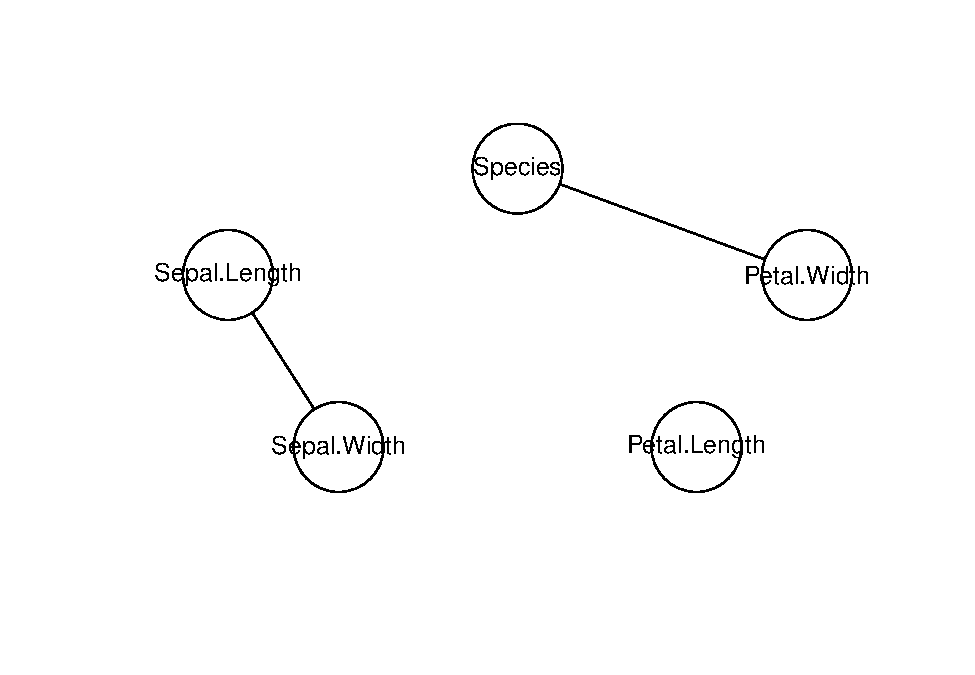
\includegraphics{BN_Ass2_files/figure-latex/unnamed-chunk-12-2.pdf}
\end{figure}

\begin{Shaded}
\begin{Highlighting}[]
\NormalTok{NewIrisNetHc1 <-}\StringTok{ }\KeywordTok{tabu}\NormalTok{(NewIris)}
\NormalTok{NewIrisNetGs1 <-}\StringTok{ }\KeywordTok{iamb}\NormalTok{(NewIris)}

\NormalTok{NewIrisNetHc1}
\end{Highlighting}
\end{Shaded}

\begin{verbatim}
## 
##   Bayesian network learned via Score-based methods
## 
##   model:
##    [Sepal.Width][Petal.Width|Sepal.Width][Species|Petal.Width]
##    [Petal.Length|Species][Sepal.Length|Petal.Length]
##   nodes:                                 5 
##   arcs:                                  4 
##     undirected arcs:                     0 
##     directed arcs:                       4 
##   average markov blanket size:           1.60 
##   average neighbourhood size:            1.60 
##   average branching factor:              0.80 
## 
##   learning algorithm:                    Tabu Search 
##   score:                                 BIC (disc.) 
##   penalization coefficient:              2.505318 
##   tests used in the learning procedure:  114 
##   optimized:                             TRUE
\end{verbatim}

\begin{Shaded}
\begin{Highlighting}[]
\NormalTok{NewIrisNetGs1}
\end{Highlighting}
\end{Shaded}

\begin{verbatim}
## 
##   Bayesian network learned via Constraint-based methods
## 
##   model:
##     [undirected graph]
##   nodes:                                 5 
##   arcs:                                  2 
##     undirected arcs:                     2 
##     directed arcs:                       0 
##   average markov blanket size:           0.80 
##   average neighbourhood size:            0.80 
##   average branching factor:              0.00 
## 
##   learning algorithm:                    IAMB 
##   conditional independence test:         Mutual Information (disc.) 
##   alpha threshold:                       0.05 
##   tests used in the learning procedure:  32 
##   optimized:                             TRUE
\end{verbatim}

\subsubsection{Values of hartemink}\label{values-of-hartemink}

\begin{Shaded}
\begin{Highlighting}[]
\NormalTok{for( bins in }\KeywordTok{c}\NormalTok{(}\DecValTok{3}\NormalTok{,}\DecValTok{5}\NormalTok{,}\DecValTok{7}\NormalTok{))\{}
\NormalTok{tmp=}\KeywordTok{discretize}\NormalTok{(iris[-}\DecValTok{5}\NormalTok{], }\DataTypeTok{method =} \StringTok{'hartemink'}\NormalTok{,}\DataTypeTok{ibreaks=}\NormalTok{bins) }
\NormalTok{NewIris =}\StringTok{ }\KeywordTok{cbind}\NormalTok{(tmp,iris[}\DecValTok{5}\NormalTok{]) }

\NormalTok{IrisNetsb <-}\StringTok{ }\KeywordTok{tabu}\NormalTok{(NewIris)}

\KeywordTok{print}\NormalTok{(IrisNetsb)}
\NormalTok{\}}
\end{Highlighting}
\end{Shaded}

\begin{verbatim}
## 
##   Bayesian network learned via Score-based methods
## 
##   model:
##    [Sepal.Width][Petal.Width|Sepal.Width][Species|Petal.Width]
##    [Petal.Length|Species][Sepal.Length|Petal.Length]
##   nodes:                                 5 
##   arcs:                                  4 
##     undirected arcs:                     0 
##     directed arcs:                       4 
##   average markov blanket size:           1.60 
##   average neighbourhood size:            1.60 
##   average branching factor:              0.80 
## 
##   learning algorithm:                    Tabu Search 
##   score:                                 BIC (disc.) 
##   penalization coefficient:              2.505318 
##   tests used in the learning procedure:  106 
##   optimized:                             TRUE 
## 
## 
##   Bayesian network learned via Score-based methods
## 
##   model:
##    [Sepal.Length][Petal.Length|Sepal.Length][Petal.Width|Petal.Length]
##    [Species|Petal.Width][Sepal.Width|Species]
##   nodes:                                 5 
##   arcs:                                  4 
##     undirected arcs:                     0 
##     directed arcs:                       4 
##   average markov blanket size:           1.60 
##   average neighbourhood size:            1.60 
##   average branching factor:              0.80 
## 
##   learning algorithm:                    Tabu Search 
##   score:                                 BIC (disc.) 
##   penalization coefficient:              2.505318 
##   tests used in the learning procedure:  106 
##   optimized:                             TRUE 
## 
## 
##   Bayesian network learned via Score-based methods
## 
##   model:
##    [Sepal.Length][Petal.Length|Sepal.Length][Petal.Width|Petal.Length]
##    [Sepal.Width|Petal.Width][Species|Petal.Width]
##   nodes:                                 5 
##   arcs:                                  4 
##     undirected arcs:                     0 
##     directed arcs:                       4 
##   average markov blanket size:           1.60 
##   average neighbourhood size:            1.60 
##   average branching factor:              0.80 
## 
##   learning algorithm:                    Tabu Search 
##   score:                                 BIC (disc.) 
##   penalization coefficient:              2.505318 
##   tests used in the learning procedure:  114 
##   optimized:                             TRUE
\end{verbatim}

\begin{Shaded}
\begin{Highlighting}[]
\NormalTok{for( bins in }\KeywordTok{c}\NormalTok{(}\DecValTok{3}\NormalTok{,}\DecValTok{5}\NormalTok{,}\DecValTok{7}\NormalTok{))\{}
\NormalTok{tmp=}\KeywordTok{discretize}\NormalTok{(iris[-}\DecValTok{5}\NormalTok{], }\DataTypeTok{method =} \StringTok{'hartemink'}\NormalTok{,}\DataTypeTok{ibreaks=}\NormalTok{bins) }
\NormalTok{NewIris =}\StringTok{ }\KeywordTok{cbind}\NormalTok{(tmp,iris[}\DecValTok{5}\NormalTok{]) }

\NormalTok{IrisNetcb <-}\StringTok{ }\KeywordTok{iamb}\NormalTok{(NewIris)}

\KeywordTok{print}\NormalTok{(IrisNetcb)}
\NormalTok{\}}
\end{Highlighting}
\end{Shaded}

\begin{verbatim}
## 
##   Bayesian network learned via Constraint-based methods
## 
##   model:
##     [undirected graph]
##   nodes:                                 5 
##   arcs:                                  2 
##     undirected arcs:                     2 
##     directed arcs:                       0 
##   average markov blanket size:           0.80 
##   average neighbourhood size:            0.80 
##   average branching factor:              0.00 
## 
##   learning algorithm:                    IAMB 
##   conditional independence test:         Mutual Information (disc.) 
##   alpha threshold:                       0.05 
##   tests used in the learning procedure:  33 
##   optimized:                             TRUE 
## 
## 
##   Bayesian network learned via Constraint-based methods
## 
##   model:
##     [undirected graph]
##   nodes:                                 5 
##   arcs:                                  4 
##     undirected arcs:                     4 
##     directed arcs:                       0 
##   average markov blanket size:           1.60 
##   average neighbourhood size:            1.60 
##   average branching factor:              0.00 
## 
##   learning algorithm:                    IAMB 
##   conditional independence test:         Mutual Information (disc.) 
##   alpha threshold:                       0.05 
##   tests used in the learning procedure:  42 
##   optimized:                             TRUE 
## 
## 
##   Bayesian network learned via Constraint-based methods
## 
##   model:
##     [partially directed graph]
##   nodes:                                 5 
##   arcs:                                  3 
##     undirected arcs:                     1 
##     directed arcs:                       2 
##   average markov blanket size:           1.60 
##   average neighbourhood size:            1.20 
##   average branching factor:              0.40 
## 
##   learning algorithm:                    IAMB 
##   conditional independence test:         Mutual Information (disc.) 
##   alpha threshold:                       0.05 
##   tests used in the learning procedure:  36 
##   optimized:                             TRUE
\end{verbatim}

\subsection{BC Dataset}\label{bc-dataset}

\subsubsection{values depending on size}\label{values-depending-on-size}

\begin{Shaded}
\begin{Highlighting}[]
\NormalTok{for(part in }\KeywordTok{c}\NormalTok{(}\DecValTok{1}\NormalTok{,}\DecValTok{2}\NormalTok{,}\DecValTok{10}\NormalTok{))\{}
    \NormalTok{ind =}\StringTok{ }\KeywordTok{sample}\NormalTok{(}\DecValTok{1}\NormalTok{:(}\KeywordTok{nrow}\NormalTok{(a)/part))}
    \NormalTok{BC <-}\StringTok{ }\NormalTok{a[ind,]}
    
    \NormalTok{BC_cbl <-}\StringTok{ }\KeywordTok{tabu}\NormalTok{(BC)}
    
    \KeywordTok{print}\NormalTok{(BC_cbl)}
\NormalTok{\}}
\end{Highlighting}
\end{Shaded}

\begin{verbatim}
## 
##   Bayesian network learned via Score-based methods
## 
##   model:
##    [BreastDensity][Age][BC|Age][Location|BC][Mass|BreastDensity:BC][AD|BC]
##    [Metastasis|BC][MC|BC][Size|Mass][Shape|Mass][FibrTissueDev|AD]
##    [LymphNodes|Metastasis][SkinRetract|BC:FibrTissueDev]
##    [NippleDischarge|BC:FibrTissueDev][Spiculation|FibrTissueDev]
##    [Margin|Mass:Spiculation]
##   nodes:                                 16 
##   arcs:                                  18 
##     undirected arcs:                     0 
##     directed arcs:                       18 
##   average markov blanket size:           2.62 
##   average neighbourhood size:            2.25 
##   average branching factor:              1.12 
## 
##   learning algorithm:                    Tabu Search 
##   score:                                 BIC (disc.) 
##   penalization coefficient:              4.951744 
##   tests used in the learning procedure:  960 
##   optimized:                             TRUE 
## 
## 
##   Bayesian network learned via Score-based methods
## 
##   model:
##    [BreastDensity][Age][BC|Age][Location|BC][Mass|BreastDensity:BC][AD|BC]
##    [Metastasis|BC][MC|BC][Size|Mass][Shape|Mass][FibrTissueDev|AD]
##    [LymphNodes|Metastasis][SkinRetract|BC:FibrTissueDev]
##    [NippleDischarge|BC:FibrTissueDev][Spiculation|FibrTissueDev]
##    [Margin|Mass:Spiculation]
##   nodes:                                 16 
##   arcs:                                  18 
##     undirected arcs:                     0 
##     directed arcs:                       18 
##   average markov blanket size:           2.62 
##   average neighbourhood size:            2.25 
##   average branching factor:              1.12 
## 
##   learning algorithm:                    Tabu Search 
##   score:                                 BIC (disc.) 
##   penalization coefficient:              4.60517 
##   tests used in the learning procedure:  960 
##   optimized:                             TRUE 
## 
## 
##   Bayesian network learned via Score-based methods
## 
##   model:
##    [BreastDensity][Location][FibrTissueDev][NippleDischarge|FibrTissueDev]
##    [Spiculation|FibrTissueDev][BC|NippleDischarge][Age|BC][Mass|BC]
##    [AD|BC:FibrTissueDev][Metastasis|BC][MC|BC]
##    [SkinRetract|BC:FibrTissueDev][Size|Mass][Shape|Mass]
##    [LymphNodes|Metastasis][Margin|Mass:Spiculation]
##   nodes:                                 16 
##   arcs:                                  16 
##     undirected arcs:                     0 
##     directed arcs:                       16 
##   average markov blanket size:           2.25 
##   average neighbourhood size:            2.00 
##   average branching factor:              1.00 
## 
##   learning algorithm:                    Tabu Search 
##   score:                                 BIC (disc.) 
##   penalization coefficient:              3.800451 
##   tests used in the learning procedure:  641 
##   optimized:                             TRUE
\end{verbatim}

\begin{Shaded}
\begin{Highlighting}[]
\NormalTok{for(part in }\KeywordTok{c}\NormalTok{(}\DecValTok{1}\NormalTok{,}\DecValTok{2}\NormalTok{,}\DecValTok{10}\NormalTok{))\{}
    \NormalTok{ind =}\StringTok{ }\KeywordTok{sample}\NormalTok{(}\DecValTok{1}\NormalTok{:(}\KeywordTok{nrow}\NormalTok{(a)/part))}
    \NormalTok{BC <-}\StringTok{ }\NormalTok{a[ind,]}
    
    \NormalTok{BC_sbl <-}\StringTok{ }\KeywordTok{iamb}\NormalTok{(BC)}
    \KeywordTok{print}\NormalTok{(BC_sbl)}

\NormalTok{\}}
\end{Highlighting}
\end{Shaded}

\begin{verbatim}
## 
##   Bayesian network learned via Constraint-based methods
## 
##   model:
##     [partially directed graph]
##   nodes:                                 16 
##   arcs:                                  13 
##     undirected arcs:                     7 
##     directed arcs:                       6 
##   average markov blanket size:           2.12 
##   average neighbourhood size:            1.62 
##   average branching factor:              0.38 
## 
##   learning algorithm:                    IAMB 
##   conditional independence test:         Mutual Information (disc.) 
##   alpha threshold:                       0.05 
##   tests used in the learning procedure:  592 
##   optimized:                             TRUE 
## 
## 
##   Bayesian network learned via Constraint-based methods
## 
##   model:
##     [partially directed graph]
##   nodes:                                 16 
##   arcs:                                  13 
##     undirected arcs:                     7 
##     directed arcs:                       6 
##   average markov blanket size:           2.12 
##   average neighbourhood size:            1.62 
##   average branching factor:              0.38 
## 
##   learning algorithm:                    IAMB 
##   conditional independence test:         Mutual Information (disc.) 
##   alpha threshold:                       0.05 
##   tests used in the learning procedure:  619 
##   optimized:                             TRUE 
## 
## 
##   Bayesian network learned via Constraint-based methods
## 
##   model:
##     [partially directed graph]
##   nodes:                                 16 
##   arcs:                                  12 
##     undirected arcs:                     7 
##     directed arcs:                       5 
##   average markov blanket size:           2.00 
##   average neighbourhood size:            1.50 
##   average branching factor:              0.31 
## 
##   learning algorithm:                    IAMB 
##   conditional independence test:         Mutual Information (disc.) 
##   alpha threshold:                       0.05 
##   tests used in the learning procedure:  596 
##   optimized:                             TRUE
\end{verbatim}

\subsection{NHL dataset}\label{nhl-dataset}

\subsubsection{Values of the networks}\label{values-of-the-networks}

INSERTXXX

\newpage

\section{list of figures}\label{list-of-figures}

\listoffigures
\newpage

\section{references}\label{references}

\twocolumn

Sing, Tobias, Oliver Sander, Niko Beerenwinkel, and Thomas Lengauer.
2005. ``ROCR: visualizing Classifier Performance in R.''
\emph{Bioinformatics (Oxford, England)} 21 (20): 3940--1.
doi:\href{http://dx.doi.org/10.1093/bioinformatics/bti623}{10.1093/bioinformatics/bti623}.
\url{http://bioinformatics.oxfordjournals.org/content/21/20/3940.abstract}.

\end{document}
